\section{Decentralized Unstructured Architectures}
\label{section:unstructured}

This section is dedicated to the unstructured P2P architectures. In the next
paragraphs, algorithms for tackling the topology mismatch problem on such
networks are discussed, analyzed and categorized based on the use of the
overlay structure, message forwarding approach for peer communication and
techniques proposed for detecting proximity in order to optimize overlay
topology.

% TODO: READ A Near-Optimal Algorithm Attacking the Topology Mismatch Problem in
%Unstructured Peer-to-Peer Networks (This is an Approximation alg for Top-mis
%problem)

%%%%%%%%%%%%%%%%%%%%%%%%%%%%%%%%%%%%%%%%%%%%%%%%%%%%%%%%%%%%%%%%%%%%%%%%%%%%%%%%
%
% TODO: HOW CAN UNSTRUCTURED SCHEMES BE REFINED
%
%For this reasons, efforts have been placed for optimizing the efficiency of
%decentralized unstructured peer-to-peer networks. Research mainly focuses on
%\begin{inparaenum}[\itshape i\upshape)]
%  \item reducing unnecessary, redundant communication traffic, and
%  \item exploiting physical locality to reduce communication response.
%\end{inparaenum}
%The goal can be achieved at, both, the application-level network as well as the
%underlying physical one. In the first case by refining the message relay
%techniques, while in the second one, by adaptively reconstructing the
%application network to map as well as possible to the the physical network.
%
%%%%%%%%%%%%%%%%%%%%%%%%%%%%%%%%%%%%%%%%%%%%%%%%%%%%%%%%%%%%%%%%%%%%%%%%%%%%%%%%


\subsection{Algorithms for Unstructured Architectures}

% BROADCAST OPTIMIZATION

%%%%%%%%%%%%%%%%%%%%%%%%%%%%%%%%%%%%%%%%%%%%%%%%%%%%%%%%%%%%%%%%%%%%%%%%%%%%%%%%
\subsubsection{Improving search in peer-to-peer networks}

% \begin{figure}[ht]
% \centering
% \subfigure[Iterative deepening with three levels.] {
%   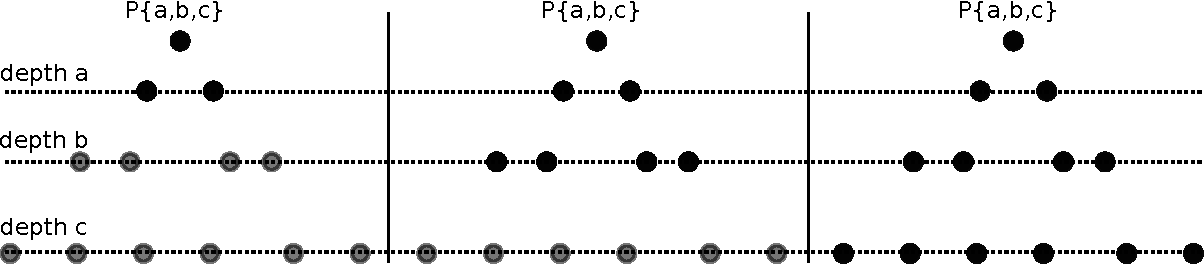
\includegraphics[scale=0.4]{img/algorithms/iterative_deepening}
%   \label{figure:dbfs:iterdeep}
% }\qquad\qquad
% \subfigure[Directed BFS.] {
%   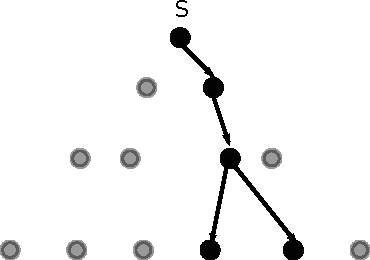
\includegraphics[scale=0.4]{img/algorithms/directed_bfs}
%   \label{figure:dbfs:dbfs}
% }\qquad\qquad
% \subfigure[Local indices with radius size equal to $2$.] {
%   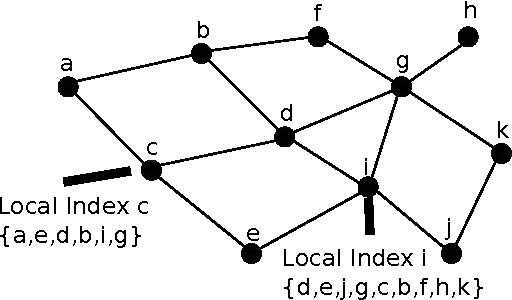
\includegraphics[scale=0.4]{img/algorithms/local_indices}
%   \label{figure:dbfs:localindx}
% }
% \caption{Improving search in P2P networks}
% \label{figure:dbfs}
% \end{figure}

\cite{YG-M2002} proposes an easy to implement and practical solution to the
inefficiency of Gnutella's ``blind flooding'' approach. The paper introduces
three different forwarding methods, namely \emph{iterative deepening},
\emph{directed BFS}, and \emph{local indices}.

In iterative deepening, %(see Figure~\ref{figure:dbfs:iterdeep})
the search is
performed on a BFS tree with multiple preset depths. The depth limit is
iteratively increased by the source node for each query, based on the quality of
the results. The source node may issue a new request with increased depth limit
that will trigger the nodes at the last depth level to resume the search. The
iterative approach avoids restarting the whole search process from scratch at
each iteration and reduces the load of the nodes on the upper levels of the
tree. Its major drawback is the delay between successive iterations, as the
source node needs to examine the results at each iteration before deciding to
quit or resume the query.

The directed BFS%, as shown in Figure~\ref{figure:dbfs:dbfs},
tries to avoid this delay by forwarding the query messages only to a selected
set of neighbors, in which the selection criteria varies from the number of
results received previously, distance in terms of hops, bandwidth, or the query
load of the neighbor.

In local indices%, as shown in Figure~\ref{figure:dbfs:localindx},
each node
indexes data within a radius of $r$ hops and uses this local index to answer
queries on behalf of them without generating additional traffic. Local indices
greatly reduce the aggregate bandwidth usage of the network and improves query
efficiency, however, updating the indices in cases with frequent node joins and
leaves introduces a serious overhead to the system if the radius is kept broad.

% \begin{center}
% \begin{tabular}{ccc}
% \textbf{Efficiency} & \textbf{Overhead} & \textbf{Scalability} \\
% \hline
% Iterative Deepening & ? & ? & ?
% Directed BFS & ? & ? & ?
% Local Indices & ? & ? & ?
% \end{tabular}
% \end{center}
\begin{center}
\begin{tabular}{rccc}
\multicolumn{1}{r}{} &
\multicolumn{1}{c}{\emph{Efficiency}} &
\multicolumn{1}{c}{\emph{Overhead}} &
\multicolumn{1}{c}{\emph{Scalability}}
\\
\cline{2-4}
\emph{Iterative Deepening} &
% needs recalculation in every iteration step
% extra delay imposed in a high churn environment that prohibits the algorithm
% to start from the last level of nodes and results in a restart of the whole
% process
low &
% the process in not started from the beginning at each iteration step
low &
% 
medium \\
\emph{Directed BFS} &
% Better time to satisfaction compared to iterative deepening
medium &
% Better quality and quicker results mean more aggregate bandwidth and
% processing power needs to be consumed since more nodes are involved (death
% spirral).
medium &
% BFS is Gnutella's non efficient communication method
medium \\
\emph{Local Indices} &
% efficiency is enhanced greatly since data pointers are replicated across the
% network
high &
% updating indices is a time and resource consuming process.
medium &
% the scalability is constrained by the indices update in a highly dynamic
% environment (high churn)
medium \\
\end{tabular}
\end{center}

%%%%%%%%%%%%%%%%%%%%%%%%%%%%%%%%%%%%%%%%%%%%%%%%%%%%%%%%%%%%%%%%%%%%%%%%%%%%%%%%
\paragraph*{ \bf Delay Aware P2P System}
A new \emph{Delay Aware P2P System (DAPS)} is introduced in \cite{ZL2005}. Its
main goal is to reduce the time of a look-up request by dividing the routing
tables of peers into several sectors of increasing delay. The source node
emitting the query message defines a delay boundary or the \emph{pruning
factor} in the paper's context. Request messages are then forwarded only to
nodes whose delay is less than or equal that boundary. With the clustered
routing tables and the loose organization of DAPS' overlay network it is
considered by is between structured and unstructured.

% TODO: MAYBE REVIEW THE EVALUATION
\begin{center}
\begin{tabular}{ccc}
\emph{Efficiency} & \emph{Overhead} & \emph{Scalability} \\
\hline
%
low &
%
low &
%
medium
\end{tabular}
\end{center}

%%%%%%%%%%%%%%%%%%%%%%%%%%%%%%%%%%%%%%%%%%%%%%%%%%%%%%%%%%%%%%%%%%%%%%%%%%%%%%%%
\subsubsection{Gia}
\emph{Gia} \cite{CRBLS2003} is an effort to solve the scalability
problem of the unstructured P2P file sharing systems, in particular Gnutella.
The main novelty in the design of Gia is the replacement of the blind flooding
approach of Gnutella with random walks \cite{lv_randomwalks_2002}. Although
random walks is a step in the right direction, issuing only a single copy of the
query within the network reduces the search scope, thus affecting negatively the
success rate of the query.  In order to overcome this limitation, Gia introduces
a token-based flow control mechanism, which is essentially an intelligent flow
control algorithm that gradually redirects the queries to nodes which are more
likely to answer. In order to prevent overloading of nodes with query requests,
Gia uses a token-based flow control algorithm in which each node announces the
number of query requests it can handle in terms of tokens to its neighbors, so
that neighbors only forward query requests to nodes that they previously
received tokens from. Gia also acknowledges the heterogeneity in peer bandwidth,
processing power, disk speed, etc, of the nodes in P2P networks and uses this
information when connecting nodes to each other and by using a topology
adaptation algorithm, Gia ensures that high capacity nodes have high degrees and
low capacity nodes are within short proximity to high capacity ones.
% TODO: THIS FOLLOWING REMARK SOUNDS LIKE THE ALGORITHM SHOULDN'T BE IN THIS
%       SURVEY AFTER ALL!!
Although the topology adaptation algorithm Gia uses improves the scalability of
the network, it does not help much in solving the topology mismatch problem,
since it does not consider the underlying physical topology.

%
%More specifically, there are four key components in the design of
%\emph{Gia} which are summarized bellow:
%\begin{enumerate}
%  \item A \emph{dynamic topology adaptation} protocol that puts
%participating nodes within short reach of high capacity nodes so that these
%\emph{high-degree} nodes, which due to their high connectivity receive most of
%the queries, actually have the capacity to handle them.
%  \item An \emph{active flow control} scheme is used to avoid overloaded
% hot-spots. Heterogeneity is detected and flow control tokens are given to
%nodes based on the available capacity.
%  \item Every node maintains pointers to to the content that is offered by
% their immediate neighbors, creating a \emph{one-hop replication} of pointers,
%scheme.
%  \item A \emph{search protocol} based on random walks, that is biased towards
% directing queries to high-capacity nodes that are typically best able to
%answer these queries.
%\end{enumerate}
%

\begin{center}
\begin{tabular}{ccc}
\emph{Efficiency} & \emph{Overhead} & \emph{Scalability} \\
\hline
% Drastically reduces the search scope.
low &
% Only one copy of the query is issued to the network.
% A token based flow control mechanism redirects queries to nodes that are most
% likely to fulfill them.
low &
% Even thought the low overhead scalability is reduced by the reducing of
% search scope.
medium
\end{tabular}
\end{center}

% \begin{center}
% \begin{tikzpicture}
% \begin{axis}[
%   ybar,
%    symbolic x coords={
%      Efficiency,
%      Overhead,
%      Scalability
%    },
%    symbolic y coords={lo, med, hi},
%    x tick label style={rotate=45,anchor=east},
%    xtick=data, ytick=data
% ]

% \addplot coordinates {
%   (Efficiency,lo)
%   (Overhead,lo)
%   (Scalability,lo)
% };

% \end{axis}
% \end{tikzpicture}
% \end{center}



%%%%%%%%%%%%%%%%%%%%%%%%%%%%%%%%%%%%%%%%%%%%%%%%%%%%%%%%%%%%%%%%%%%%%%%%%%%%%%%%
\subsubsection{Distributed Cycle Minimization Protocol (DCMP)}
We have already discussed that blind flooding mechanism broadcasts messages with
no real targeting, many times to a direction far from the path that can
ultimately fulfill the query request. Another problem with topology unaware
systems is the duplication of messages due to cycles, even along the correct
forwarding path. The authors of \cite{ZKB2008} focused on that exact deficiency
of overlay networks and introduced Distributed Cycle Minimization Protocol
(DCMP), a dynamic, fully distributed method to remove cycles without sacrificing
overlay connectivity, resilience and other important properties of unstructured
architectures by avoiding a hierarchical organization of peers. In DCMP, once a
cycle is detected, the most powerful node in that cycle is elected as the
\emph{Gate Peer} and the cycle is then broken at a strategic place so that it
will result in the minimization of the distance between the Gate Peer and all
other nodes that participated in that cycle. The process is managed by using two
special message types namely \emph{Information Collection (IC)} and \emph{Cut
Message (CM)}. One disadvantage of DCMP is that since the distance a forwarded
message can travel is limited by the TTL value, which is practically $7$ in most
cases DCMP cannot detect cycles formed by more than 7 peers. Even though cycle
elimination improves the network performance, it does not actually solve the
topology mismatch problem.

%
%\subsection{Distributed Cycle Minimization Protocol}
%
%\paragraph{}
%The first step after detecting a duplicate message by some peer is to gather
% information from all peers in the cycle using a new type of control message
%called \emph{Information Collecting Message} or \emph{ICM}. ICM contains:
%\begin{inparaenum}[\itshape i\upshape)]
%  \item a \emph{GUID}\footnote{Globally Unique Identifier assigned to every
% query message generated by any node.} field same as the one of the duplicate
%message,
%  \item \emph{DetectionID} field which represents the direction of the
% connection where the duplicate was identified\footnote{This ensures the
%uniqueness of the ICM messages because as it travels through many cyclic paths,
%multiple peers will detect the duplicates and initiate an ICM message.}, and
%  \item \emph{Node Information Vector (NIV)} which contains information
% (bandwidth, CPU power, etc) about peers that propagated the ICM.
%\end{inparaenum}
%
%\paragraph{}
%Suppose $A$ detected the duplicate as depicted in Figure~\ref{figure:dcmp}. It
% then emits an ICM to $B$ and $F$, that initially contains information only
%about itself. Each peer that receives the ICM, appends its information and
%propagates it along the reverse path of the original message. Since two copies
%of ICM are sent, at some point, a peer, say peer $D$, will receive a duplicate
%ICM. Using the information in the NIVs of the ICMs, $D$, decides to cut (for
%example) the EF connection. To inform the other peers about its decision, it
%emits a \emph{Cut Message (CM)} which contains the GUID and DetectionID of the
%corresponding ICM and an additional field that identifies the connection to be
%cut. $D$, then, forwards the CM in the reverse directions from where the ICM
%arrived. Similarly CMs received by any peer are propagated toward the reverse
%path of the corresponding ICM. Eventually, either peer $E$ or peer $F$ will
%receive the CM and cut the connection, thus eliminating the cycle.
%
%Receiving a duplicate ICM denotes the existence of a cycle. The opposite is not
% true though. For example, if the cycle contains $2 \times TTL$ edges, it will
%not be detected, because the ICM messages will be discarded before they locate
%it. There is a trade-off between preserving the connectivity of the network and
%minimizing the duplicates that makes such a possibility to be safely ignored.
%
%\begin{figure}
%\centering
%  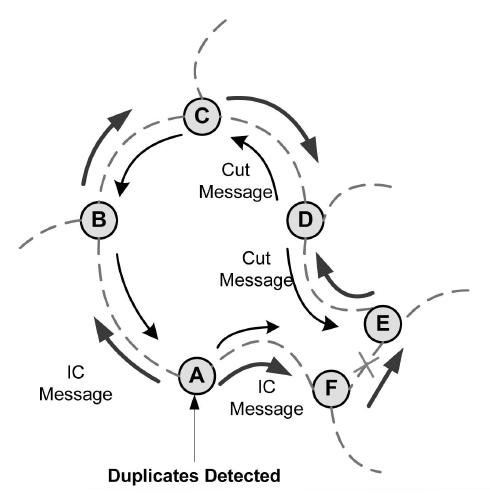
\includegraphics[scale=0.4]{img/dcmp.jpeg}
%\caption{Cycle elimination methods in DCMP}
%\label{figure:dcmp}
%\end{figure}
%
%\paragraph{}

%
% TODO: SOME DISCUSSION
%
%Actually, the duplicate packet problem seems to hurt more the active nodes;
%those with higher capacities and bandwidth that contribute the most to the
%network.
%

\begin{center}
\begin{tabular}{ccc}
\emph{Efficiency} & \emph{Overhead} & \emph{Scalability} \\
\hline
% It return more result than LTM according to experiments in
% \cite{ZKB2008}
medium &
% Duplicates are an important fraction of the redundant overhead imposed by
% topology mismatch and thus DCMP minimizes this as possible.
% The control overhead is also one to two orders of magnitude less than LTM due
% to its ``lazy'' broadcasting of control messages (as opposed to LTM's periodic
% approach) - \cite{ZKB2008}
low &
% fully distributed method
high
\end{tabular}
\end{center}

%       CACHING

%%%%%%%%%%%%%%%%%%%%%%%%%%%%%%%%%%%%%%%%%%%%%%%%%%%%%%%%%%%%%%%%%%%%%%%%%%%%%%%%
\subsubsection{Replication Strategies in Unstructured Peer-to-Peer Networks}
\cite{CS2002} aim to improve the inefficient blind search algorithm by
replicating the data in a P2P network. The main intuition behind the
idea of replication, or using cached copies, is that as the number of copies for
each item increases in the network, it would be easier for a search algorithm,
even a random one, to locate these items. In order to analyze the feasibility of
such an approach, the authors investigate three different replication
strategies, namely uniform, proportional, and square root allocation. In the
uniform model, the copies of items are uniformly replicated in the network,
while in the proportional model, the items are replicated based on their query
rate, so that frequently queried items are replicated more. The square root
allocation is a strategy proposed by Cohen and Shenker, which is a model between
the uniform and proportional allocation.  In order to evaluate the outcome of
the replication models, the overall costs of successful and unsuccessful
searches in the network are compared. Results argue that the uniform allocation
model minimizes the maximum search size, therefore reduces the time spent on an
unsuccessful search. The proportional model, on the other hand, promotes the
more frequently queried items by replicating them more, therefore decreases the
search time for popular items, but suffers when needing to locate the rare
items. The authors also claim that the expected successful search size is the
same for uniform and proportional models, and any approach between them would
always behave much better. Therefore they propose the square root allocation
approach, which is a replication strategy that minimizes the expected search
size of successful queries in P2P networks.

\begin{center}
\begin{tabular}{rccc}
\multicolumn{1}{r}{} &
\multicolumn{1}{c}{\emph{Efficiency}} &
\multicolumn{1}{c}{\emph{Overhead}} &
\multicolumn{1}{c}{\emph{Scalability}}
\\
\cline{2-4}
\emph{Uniform Replication} &
% Proportional and Uniform are the worst “reasonable” strategies
low &
% When item is created, replicate its key in a fixed number of hosts.
low &
%
medium \\
\emph{Proportional Replication} &
% Proportional and Uniform are the worst “reasonable” strategies
low &
% for each query, replicate the key in a fixed number of hosts (need to know or
% estimate the query rate)
medium &
%
low \\
\emph{Square Root Replication Allocation} &
% All (strictly) in-between strategies are (strictly) better than Uniform and
% Proportional - replication theory
medium &
% Assuming that each query keeps track of the search size then each time a query
% is finished the object is copied to a number of sites proportional to the
% number of probes that the search required.
medium &
% e.g. path replication is easy to scale, just detect the path along which the
% query ultimately got fulfilled
medium \\
\end{tabular}
\end{center}

%%%%%%%%%%%%%%%%%%%%%%%%%%%%%%%%%%%%%%%%%%%%%%%%%%%%%%%%%%%%%%%%%%%%%%%%%%%%%%%%
% \subsubsection{Tracing a large-scale Peer to Peer System: an hour in the life
% of Gnutella}
% TODO: This looks better as an analysis for the unstructured networks in
% general and specifically for caching, so it doesn't seem to contribute any
% new approach.... At least we do not present anything here. Maybe we need to
% revisit the paper itself once more
% \cite{Markatos02} analyses Gnutella network traffic traces and by concluding
% there is locality among query requests, proposes a caching algorithm that tries
% to exploit these findings . The analysis of the trace data reveals other
% important facts about the structure of the Gnutella network and the query data.
% One significant observation is that the geographic locations of clients do not
% have a correlation with the number of query requests they receive. This is an
% obvious result of the topology mismatch problem caused by the overlay structure
% of the Gnutella network. Gnutella's traffic is observed to be bursty both for
% query requests and query responses, even in longer intervals. It is observed
% that a peer receives 50 query messages per second on average! Moreover nine out
% of ten queries do not generate any response due to the inefficient design of
% the Gnutella network. When developing a caching system to exploit locality,
% applying an approach similar to web caching does not fit well with P2P systems.
% Caches in P2P systems not only have to consider the query string, but also
% the TTL value, the source of the query, and the time of the query as well.  In
% general, even though optimum caching is hard to achieve, it is reported that
% it improves the overall performance of the Gnutella network.

% \begin{center}
% \begin{tabular}{ccc}
% \emph{Efficiency} & \emph{Overhead} & \emph{Scalability} \\
% \hline
%
% ? &
%
% ? &
%
% ?
% \end{tabular}
% \end{center}


%       OVERLAY OPTIMIZATION

%%%%%%%%%%%%%%%%%%%%%%%%%%%%%%%%%%%%%%%%%%%%%%%%%%%%%%%%%%%%%%%%%%%%%%%%%%%%%%%%
\subsubsection{Narada}

% \begin{figure}[ht]
% \centering
% \subfigure[Underlying network with edge costs.] {
%   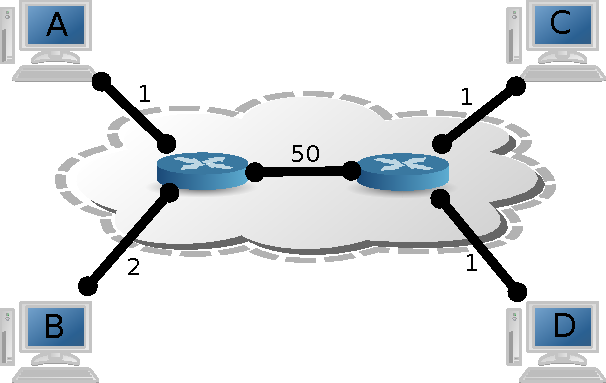
\includegraphics[scale=0.4]{img/algorithms/narada}
%   \label{figure:narada:underlying}
% }\qquad\qquad
% \subfigure[Peer A sends a message to the rest using regular broadcast.] {
%   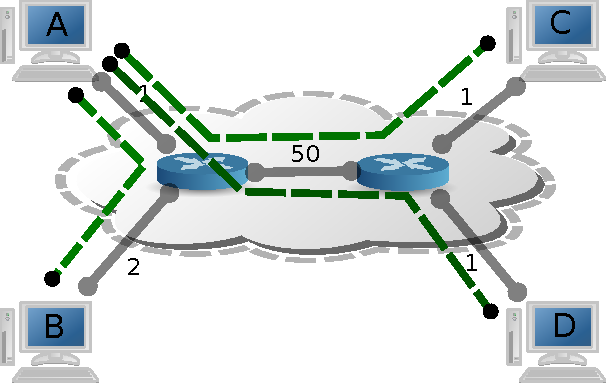
\includegraphics[scale=0.4]{img/algorithms/narada2}
%   \label{figure:narada:regu}
% }\qquad\qquad
% \subfigure[Peer A sends a message to the rest using end system multi-cast.] {
%   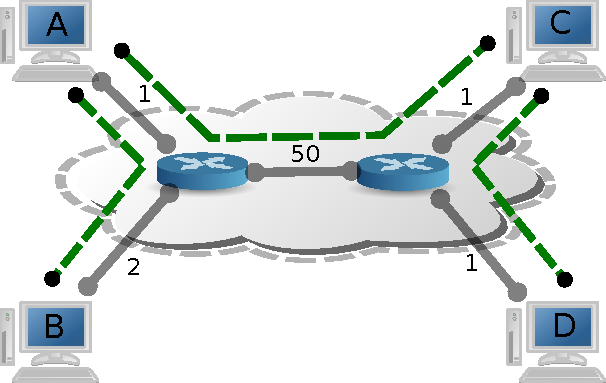
\includegraphics[scale=0.4]{img/algorithms/narada3}
%   \label{figure:narada:multicast}
% }
% \caption{A visualization of the Narada protocol.}
% \label{figure:narada}
% \end{figure}

\emph{Narada} \cite{CRZ2000,CRSZ2001,CRSZ2002} is a generic
protocol for creating self-adapting overlay networks, that can achieve
application-layer multi-cast communication without requiring IP multi-cast
infrastructure at the network layer\footnote{
  IP multi-cast is the term referring to the method of sending IP datagrams to a
  group of receivers in a single transmission. Even though the method is
  available some years now, IP multi-cast has not taken off as anticipated since
  many believe that it violates the stateless design of the current Internet.
  For this reason it is widely deployed in contained environments like
  enterprises (i.e. IPTV applications - distance learning, video conferencing),
  commercial stock exchanges, and multimedia content delivery networks.
}. Although it was not originally designed as a P2P system nor can be considered
scalable in the contemporary sense of the term, Narada has been pioneering
(maybe along with \emph{Scattercast} \cite{C2000}) in that
it was the first to consider the feasibility of overlay-based, application
layer, services over the Internet that can take into account bandwidth and
latency properties of the physical underlying infrastructure. Additionally,
authors realized the inefficiency caused by the topology mismatch problem and
tried to encounter it by building a richer connected graph, called a
\emph{mesh}, and building per source minimum spanning trees\footnote{
  ENarada \cite{LYL2008} used Gossip protocol for the
construction
}.
%as shown in Figure~\ref{figure:narada}.
They also keep the graph and the trees
dynamically updated while nodes continue to join and leave the network.
Moreover, the protocol tries to ease the physical link stress, the overall
resource usage and the relative delay among end systems. Unfortunately, the most
important limitation of Narada is that although it works reasonably well for
small groups, it does not scale well for larger networks, therefore it is not
suitable for, potentially very large, P2P file sharing application networks.

\begin{center}
\begin{tabular}{ccc}
\emph{Efficiency} & \emph{Overhead} & \emph{Scalability} \\
\hline
%
low &
% The overhead of Narada is proportional to the multicast group size
high &
%
low
\end{tabular}
\end{center}

%%%%%%%%%%%%%%%%%%%%%%%%%%%%%%%%%%%%%%%%%%%%%%%%%%%%%%%%%%%%%%%%%%%%%%%%%%%%%%%%
\subsubsection{Adaptive Overlay Topology Optimization (AOTO)}
\emph{Adaptive Overlay Topology Optimization (AOTO)} \cite{LZXN2003} is one
of the first attempts, along with Narada, to address the topology mismatch
problem. AOTO is a distributed algorithm that works in two steps, namely
\emph{Selective Flooding} and \emph{Active Topology} to optimize the usage of
the underlying physical resources. In \emph{Selective Flooding} a minimum
spanning tree is built among each peer and its immediate neighbors so that
queries are not flooding the whole network and at the same time without
shrinking the search scope. During \emph{Active Topology}, the overlay
links are revised so that they depict the physical network topology as close as
possible. This is done independently, by each peer by replacing non-flooding
neighbors, with closer nodes. Picking a replacement out of these non-flooding
neighbors follows a random policy (called \emph{Randomized AT} algorithm in the
paper's context). For these steps a peer needs to keep track of communication
costs to all its neighbors (e.g. the network delay) as well as between any
pair of neighbors (meaning also that additional, cost probing, message types
need to be added to the Gnutella protocol). Whenever a new neighbor cost table
is received or there is a change of neighbors, the source peer has to
re-calculate the multi-cast tree and apply the randomized AT algorithm.

%\paragraph*{Selective Flooding (SF)}
%
% TODO: I DON'T REMEMBER WHY THE FOLLOWING IS MENTIONING LTM WHICH IS ANOTHER
%       ALGORITM. MAYBE THIS CAN BE USED AS A PART OF DISCUSSION AND/OR
%       COMPARISON OF AOTO AND LTM
% TODO: EDIT: LTM SEEMS A MISTAKE HERE BETTER NOT USE IT FOR DISCUSSION (THIS
%             IS AOTO)
%LTM's SF effectiveness has be proven to be detached from the different physical
% or overlay topologies. On the other hand, SF is more effective with large
%number of logical neighbors. It can reach an average optimization rate of 87.4
%percent on a logical topology with an average of 30 logical neighbors.
%
%\paragraph*{Active Topology (AT)}
%
%Different numbers of average logical neighbors has little to do with the
% effectiveness of AT. If the source has $n$ non-flooding peers, there are $n$
%potential neighbor replacements. The overhead to exhaust all $n$ possible
%replacements can be high, so in practice, after each replacement the source
%peer can decide whether it needs to find another candidate peer. This is done
%by computing the cost improvement ratio greater than some predefined
%termination threshold. The larger the threshold, the slower, in the number of
%optimization steps, the reduction of the normalized average distance. As a
%whole the average response time is significantly reduced when more optimization
%steps taken.

\begin{center}
\begin{tabular}{ccc}
\emph{Efficiency} & \emph{Overhead} & \emph{Scalability} \\
\hline
%
medium &
% tracking of communication costs to all peer's neighbors as well as between
% any pair of neighbors. Whenever a new neighbor cost table is received or
% there is a change of neighbors, the source peer has to re-calculate the
% multi-cast tree and apply the randomized AT algorithm.
high &
% needs global knowledge
medium
\end{tabular}
\end{center}

%%%%%%%%%%%%%%%%%%%%%%%%%%%%%%%%%%%%%%%%%%%%%%%%%%%%%%%%%%%%%%%%%%%%%%%%%%%%%%%%
\subsubsection{Adaptive Connection Establishment (ACE)}
\emph{Adaptive Connection Establishment (ACE)} \cite{LZXN2004} builds an
overlay multi-cast tree among each source node and the peers within a certain
diameter from the source peer and optimizes the neighbor connections that are
not in that tree. To achieve that, it calculates cost between nodes using
network delay as a metric. Each peer probes the costs with its immediate logical
neighbors and forms a \emph{neighbor cost table (NCT)} using a special
routing message type. Two neighboring peers exchange their NCTs in order for
every peer to obtain the cost between any pair of its local neighbors forming a
small overlay topology. Moreover, based on obtained NCTs a minimum spanning tree
among each peer and its immediate neighbors is built. Ultimately, physically
far away neighbors are replaced by physically close ones. Specifically, a peer
$S$ probes the distance between one of its non-flooding neighbor's neighbor,
say $G$ and $H$ respectively. Assuming that the neighbor's neighbor ($SH$) is
measured as being ``closer'' that the neighbor ($SG$), the link to the later
is cut and a new connection is established. In the opposite situation where
distance $SG$ is closer than $SH$ then if $SH$ is shorter that $GH$ then $H$ is
preserved as $S$'s new neighbor. In the case where $SH$ is larger than $SG$ and
$GH$, no connection will be established and $S$ will continue probing another
neighbor's neighbor. The above optimization is conducted within $1$-neighbor
closure (among its source peer and all its direct neighbors) but the scope can
be extended. The larger the scope, the better topology matching improvement but
also the greater the computational overhead.

%
% TODO: SOME DISCUSSION
%
%Simulations in \cite{liu_acesims_2004} show that the average scope of each
% query to cover the same scope of nodes is reduced by about 65 percent without
%losing any autonomy feature, while the average response time can be reduced by
%35 percent. Larger diameter topologies lead to better topology optimization
%rate but also to higher communication and computation overhead. It was also
%found that it is more effective in higher connectivity dense topologies.
%Compared to LTM, it comes short of convergence speed. In
%\cite{ni_mismatch_2004} shows reduction of both total traffic (90 percent) and
%response time (80 percent) to message queries without shrinking the search
%scope.Last but
%not least, it is concluded that work must be done on incorporating a more
%sophisticated selection policy for candidate non-flooding peers.
%

%In \emph{Adaptive Connection Establishment (ACE)} \cite{LZXN2004}, the
%authors extend the idea of AOTO by introducing optimizations based on the
%depths of the minimum spanning trees. But since the network delay is not
%always a reliable estimation method to detect the physical location of peers,
%the algorithm still suffers from the discrepancies caused by mis-located nodes.

\begin{center}
\begin{tabular}{ccc}
\emph{Efficiency} & \emph{Overhead} & \emph{Scalability} \\
\hline
% compared to LTM it has slow convergence speed.
medium &
% A little bit better that AOTO since the computation here is done within a
% certain diameter from the source peer
medium &
% Larger diameter topologies lead to better topology optimization
% rate but also to higher communication and computation overhead.
medium
\end{tabular}
\end{center}

%%%%%%%%%%%%%%%%%%%%%%%%%%%%%%%%%%%%%%%%%%%%%%%%%%%%%%%%%%%%%%%%%%%%%%%%%%%%%%%%
\subsubsection{Location-aware Topology Matching (LTM)}
\emph{Location-aware Topology Matching (LTM)} \cite{LLXNZ2004} proposes a
method to optimize the overlay structure of the P2P network based on the
physical topology. To achieve this, peers issue special messages called
\textit{TTL-detector}s with TTL values of 0 and 1 so that the receiving peers
discover one- and two-hop neighbor sets ($N$ and $N^2$ respectively) around
them and calculating communication costs. Calculation is achieved through
time-stamp checking, so clocks must be synchronized. The latency information
gathered is later used to evolve the overlay network into a more efficient one,
without reducing the search scope. Each node examines the latency information
among his direct neighbors and those with larger latency are put in to a
will-cut list where they remain for a certain period of time until when they are
ultimately cut and recorded to the peer's cut list. Thus, low productive
connections are dropped and replaced by more efficient ones, reducing the
latency on the overall network. Although LTM improves the overall efficiency of
the P2P network, it does not actually use real physical topology information,
just latency metrics, therefore it does not offer a guaranteed safety net for
the topology mismatch problem.

%
% TODO: SOME DISCUSSION
%
%\paragraph*{Low productive connection cutting}
%There are three cases for any peer $P$ who receives $d(i, S, v)$ multiple
% times:
%\begin{inparaenum}[\itshape i\upshape)]
%  \item $P$ receives both $d(i, S, 1)$ and $d(i, S, 0)$
%  \item $P$ receives multiple $d(i, S, 0)$s from different paths, and P
% randomly chooses to process one
%  \item $P$ receives one $d(i, S, 1)$ and multiple $d(i, S, 0)$s, and $P$
% processes $d(i, S, 1)$ and one randomly selected $d(i, S, 0)$
%\end{inparaenum}
%If the link with the largest cost is found and is a direct neighbor then the
% connection is put in a will-cut list and stays there for a certain period of
%time. If it is not, then it is handled by other peers. After that period,
%connections are cut and recorded to $P$'s cut-list.
%
%\paragraph*{Source probing}
%For a peer $P\in(N^2(S) - N(S))$ who receives only one $d(i, S, 0)$, the cost
% of $PS$ is obtained (with list look-up or probing). Then $P$ compares it with
%the cost from each hop and if $PS$ has the largest cost, $P$ will not keep this
%connection, while otherwise the connection will be created.
%
%\paragraph{}
%Supposing $n$ is the number of peers, $c_n$ is the average number of neighbors
% and $c_e$ is the average cost of logical links, then in the flooding-based
%search the traffic incurred by one query from an arbitrary peer in a
%peer-to-peer network is $O(n)$. As observed in the Gnutella network
%\cite{sripanidkulchai_gnutella_2001}, each peer issues $0.3$ queries per minute
%in average, thus the per minute traffic incurred by the network with $n$ peers
%is $O(n^2)$. Because each $d(i, S, v)$ has a TTL of $2$ in each source peer,
%the traffic for one time LTM optimization in all peers is at most $2nc_n^2c_e$.
%If each peer uses LTM $k$ times per minute, the total traffic incurred is
%$2knc_n^2c_e$. Simulation shows the best value for $k$ is $2$ or $3$. So, the
%traffic overhead caused by LTM to the network is $O(n)$.
%
%TTLj-detectors, with $j > 2$, would detect and break cycles with more than 4
% links. LTM though, does not use such detectors because detector-flood traffic
%would increase significantly, and cut links between two end-peers, could cause
%queries initiated by them to traverse a path much more expensive than the cost
%on the the cut link.
%
%\paragraph{}
%LTM disadvantages are
%\begin{inparaenum}[\itshape i\upshape)]
%  \item disagreement of measured delay due to unsynchronized clocks causes
% problems when deciding the cut positions, which can influence the network
%connectivity, and
%  \item the network delay metric mainly focuses on disabling the connections
% between peers physically far away without considering the shortcuts created by
%powerful peers.
%\end{inparaenum}
%

\begin{center}
\begin{tabular}{ccc}
\emph{Efficiency} & \emph{Overhead} & \emph{Scalability} \\
\hline
% Authors claim 75% reduction on traffic cost and about 65% reduction on query
% response time.
medium &
%
medium &
%
medium
\end{tabular}
\end{center}

%%%%%%%%%%%%%%%%%%%%%%%%%%%%%%%%%%%%%%%%%%%%%%%%%%%%%%%%%%%%%%%%%%%%%%%%%%%%%%%%
\subsubsection{Scalable Bipartite Overlay (SBO)}
\emph{Scalable Bipartite Overlay (SBO)}
\cite{LXN2004,LXN2007} reduces the overhead of creating
and maintaining a minimum spanning tree cost by randomly dividing the nodes into
two groups, namely red and white and assigning different tasks to different
groups. When a peer joins the network, it is randomly assigned with an initial
color, say red or white (separating all peers into two groups). Then the peer
that plays the role of the boot-strap host provides the joining peer with a list
of active peers along with their color information. The later uses this list to
establish connections to differently colored peers. This way, all peers form a
bipartite overlay. The white peers measure distances to neighbors (red only) by
using the network delay as a metric and report their corresponding red
neighbors. The red peers, equipped with the information of all two-hop
neighbors ($N^2$), creates minimum spanning tree of these neighbors and
assigns efficient forwarding paths. Having a minimum spanning tree with two
hops, a red peer is able to send its queries within that range. Some white
peers, though, have become non-forwarding neighbors. In this phase, such a
(white) neighbor will try to find another red peer being two hops away from its
current red neighbor to replace the later as its new neighbor. The white peers
can further optimize their positions within the overlay if this is required.

%
% TODO: SOME DISCUSSION
%
%In a static environment LTM may reduce traffic cost by around 80 to 85 percent
% while SBO reduces traffic cost between 85 and 90 percent. However, LTM  is
%proved to converge in around 2-3 steps while SBO needs 4-5 steps. Moreover LTM
%reduces response time by more than 60 percent in 3 steps while SBO needs 8. In
%a dynamic environment (10 minute average peer lifetime, 0.3 queries/sec by each
%peer) SBO and LTM reduce the average traffic cost per query (including the
%overhead due to the optimization steps) by 85 and 80 percent, respectively.
%Moreover LTM reduces the response time per query to 30 percent while SBO to 35
%percent.
%
%\cite{ni_mismatch_2004} shows SBO, achieves approximately 85 percent reduction
% on traffic cost and about 60 percent reduction on query response time.

\begin{center}
\begin{tabular}{ccc}
\emph{Efficiency} & \emph{Overhead} & \emph{Scalability} \\
\hline
% SBO reduces traffic cost between 85 and 90 percent
high &
% compared to LTM it has slower convergence speed thus incurs more, total,
% overhead.
medium &
%
medium
\end{tabular}
\end{center}

%%%%%%%%%%%%%%%%%%%%%%%%%%%%%%%%%%%%%%%%%%%%%%%%%%%%%%%%%%%%%%%%%%%%%%%%%%%%%%%%
\subsubsection{Two-Hop-Away Neighbor Comparison and Selection (THANCS)}
Work in \cite{LNXE2005,L2008} proposes a distributed heuristic
called \emph{Two-Hop-Away Neighbor Comparison and Selection (THANCS)} that
tries to minimize the overlay hop costs. THANCS is considered a \emph{local
search method}, in the sense that it targets in finding a locally optimum
solution, by exploiting knowledge within a 2-hop radius. The algorithm consists
of two main components: \emph{piggybacking neighbor distance on queries} and
\emph{neighbor comparison and selection} which are further discussed bellow.
The first component dictates peers to probe distances (using network delay
distance measuring) with its immediate neighbors and stores information
locally. This is done by introducing a special query message type, the
\emph{Piggy Message (PM)} which includes information about the neighbor
identification and measured distance. A peer $p$ constructs a PM for its
neighbor $n$, which contains $n$'s IP address and the distance between them.
When $p$ receives a query from $n$, this PM will be piggybacked to the query
message that will be then forwarded to all other neighbors of peer $p$. Upon
receiving such a query message, each of the other neighbors will detach the PM
information (it will not be further forwarded), record the $pq$ distance and
process the query as always. Selection of which incoming queries should
piggyback a PM is proposed by either \emph{pure probability-based (PPB)} or
\emph{new neighbor triggered (NNT)} policies. The second component, namely
neighbor comparison and selection, dictates peer $p$ to probe the distance to
all his known, not yet probed, two-hop neighbors ($ N^2(p)$). The distance of
$pn$ is known to $p$. Upon receiving a PM from node $n$ with the distance of
$nq$, where $q$ is a direct neighbor of $n$, $p$ chooses one of the following
two paths. First, if $q$ is a direct neighbor of $p$, then the later will check
the cost of the involved links. If the most cost-intensive link is one of $pq$
or $pn$, then it is put into a \emph{will-cut} list. If it is $nq$ then nothing
is done (since either $n$ or $q$ will have the chance to handle it themselves).
On the other hand, if $q$ is within two-hop radius from $p$, the later probes
the former (if it hasn't got the distance information yet) and again compares
distances $pq$, $pn$ and $nq$. If $pq$ is the most cost-intensive, $p$ will not
establish the connection. If it is $pn$, $p$ will establish connection $pq$ and
put $pn$ in the will-cut list. If it is $nq$, $p$ will keep the connection with
both $n$ and $q$, expecting that eventually either $n$ or $q$ will disconnect
link $nq$, later.

%
% TODO: SOME DISCUSSION
%
% \begin{inparaenum}[\itshape i\upshape)]
%   \item is completely distributed and needs no global knowledge,
%   \item presents trivial overhead compared to the query cost savings
%   \item its convergent speed of the algorithm is fast enough (faster than
% minimum spanning tree approaches) so that is effective to dynamic
% environments, and
%   \item does not shrink the search scope.
% \end{inparaenum}
%
%In a static environment THANCS has been proven to be effective; optimizing 45
% percent out of the 60 percent of mismatched paths, constructing a nearly
%optimal overlay. This leads to a 60 percent reduction in traffic cost as well
%as a 40 percent decrease in query response time. In dynamic environments
%(Gnutella 0.6/Limewire super-peer-like and Ion flat-like), THANCS saves up to
%70 percent of the traffic cost in the super-peer topology and 55 percent for
%the flat one. Average response time is also decreased by 60 and 45 percent,
%respectively. Generally, THANCS has similar performance to LTM, without needing
%synchronization. SBO, incurring half the  overhead of AOTO, reduces the traffic
%cost the most, while THANCS has lower response time and converges faster than
%SBO. THANCS is, thus, more suitable for a more dynamic environment. In
%addition, THANCS is easy to implement and its operation overhead is trivial,
%compared with the other three approaches. This design, however, has the
%limitation of not being easily extend to also support non-flooding-based
%systems.

\begin{center}
\begin{tabular}{ccc}
\emph{Efficiency} & \emph{Overhead} & \emph{Scalability} \\
\hline
% 
medium &
% trivial overhead compared to the query cost savings and its convergent speed
% is faster than minimum spanning tree approaches so less overall overhead cost.
low &
% completely distributed and needs no global knowledge,
high
\end{tabular}
\end{center}

%%%%%%%%%%%%%%%%%%%%%%%%%%%%%%%%%%%%%%%%%%%%%%%%%%%%%%%%%%%%%%%%%%%%%%%%%%%%%%%%
\subsubsection{Hops Adaptive Neighbor Discovery (HAND)}
\cite{CLZHC2006} proposes the \emph{HAND} algorithm which uses a
fully distributed triple hop adjustment strategy to address the topology
mismatch problem. The approach's ultimate goal is to shape the current overlay
graph $G$ into the \emph{Logical Communication Network (LCN)} $G^{*}$ which is
how the optimal overlay is referred in the paper's context. A formal
definition of achieving the above match is only if all peer hop sequences $(v_1,
v_2, \ldots, v_k)$ in $G$ exist in $G^{*}$ and in the same order\footnote{In
practice triple sequences $(v_1, v_2, v_3)$ are used.}. The mismatching
detection is done in the following way. Suppose we want to verify peer a
sequence, say $v_2-v_1-v_3$. A pair of probing messages are sent from $v_1$ to
$v_2$ and $v_3$. Suppose delays of $(v_1,v_2)$ and $(v_1,v_3)$ are denoted as
$x$ and $z$, respectively. When the probing message arrives to $v_2$ it forwards
it directly to $v_3$. Similarly, when the probing message arrives to $v_3$, it
forwards it directly to $v_2$. These last steps are performed in order to obtain
delays of $(v_2,v_3)$ and $(v_3,v_2)$ physical paths, respectively, denoted by
$y$. If $y=z-x\pm\varepsilon$, sequence $v_2-v_1-v_3$ is mismatched and should
be adjusted to $v_1-v_2-v_3$ by deleting edge $(v_1,v_3)$ and adding a new
$(v_2,v_3)$. If $y=x-z\pm\varepsilon$, sequence $v_2-v_1-v_3$ is mismatched and
should be adjusted to $v_1-v_3-v_2$ by deleting edge $(v_1,v_2)$ and adding a
new $(v_3,v_2)$, where $\varepsilon$ is a small positive real number denoting
additional delays caused by possible forwarding and jitter delays. The
advantages of the HAND algorithm compared to other approaches are that:
\begin{inparaenum}[\itshape i\upshape)]
  \item it does not need any clock synchronization,
  \item it is a fully distributed algorithm making it robust and reliable in
        decentralized systems,
  \item the traffic overhead of the triple hop adjustment is very low,
  \item it is applicable to dynamic peer-to-peer environments, and
  \item maintains lower query response times.
\end{inparaenum}

%
% TODO: SOME DISCUSSION
%
%Measurements conducted for evaluation purposes showed that in a static
% environment the algorithm can effectively decrease traffic cost by about 77
%percent and shorten the query response time by about 49 percent in less than
%two minutes. In a dynamic environment it shows similar behavior and with the
%size of the overlay network having little impact on the effectiveness of the
%algorithm. Compared to LTM both algorithms have almost the same traffic
%reduction rate, however on the response time reduction rate HAND has a higher
%one by about 4 percent. The traffic overhead of HAND is much less than that of
%LTM by an average of 55 percent.

\begin{center}
\begin{tabular}{ccc}
\emph{Efficiency} & \emph{Overhead} & \emph{Scalability} \\
\hline
% similar traffic reduction rate savings to LTM
medium &
% The traffic overhead of HAND is much less than that of LTM by an average of
% 55 percent.
low &
% no clock syncing needed, fully distributed and with low control overhead the
% algorithm can be considered scalable.
high
\end{tabular}
\end{center}

%%%%%%%%%%%%%%%%%%%%%%%%%%%%%%%%%%%%%%%%%%%%%%%%%%%%%%%%%%%%%%%%%%%%%%%%%%%%%%%%
% TODO: DOUBLE CHECK IF THIS ALGORITHM GOES IN THIS SECTION/SUBSECTION
\subsubsection{Adaptive Peer Selection (APS)}
Bernstein et al., contributed on the use of machine learning for building peer
selection strategies from past experience \cite{BFLZ2003}. A decision tree is
used to rate peers based on information about connection characteristics that is
collected. These can be load, bandwidth, and past uploading experience. Then a
by Markov decision process is incorporated as a mechanism to shape the policy
for switching among the peers. The problem with this approach is that the peer
selection algorithm is slow due to the learning process and the complexity of
the method.

\begin{center}
\begin{tabular}{ccc}
\emph{Efficiency} & \emph{Overhead} & \emph{Scalability} \\
\hline
% machine learning the best way to adapt the overlay 
high &
% high computation overhead for learning and very slow convergence speed for
% the learning process.
high &
%
low
\end{tabular}
\end{center}

%%%%%%%%%%%%%%%%%%%%%%%%%%%%%%%%%%%%%%%%%%%%%%%%%%%%%%%%%%%%%%%%%%%%%%%%%%%%%%%%
\subsubsection{Innocuous Topology Aware (ITA) Overlay Construction}
\cite{PRFM2009} introduces an algorithm for Innocuous Topology Aware
construction of unstructured P2P networks. The paper's proposition is twofold.
Overlay construction and search method. For the overlay construction it employs
the notion of \emph{short} and \emph{long} connections. Assuming $N$ is the
number of all network participants, $\alpha \leq 1 $ a system-wide magic number
and $x$ an $\alpha$-related latency threshold, the boot-strapping peer randomly
selects $\alpha \ast N$ close (latency bellow $x$) and
$\left( 1 - \alpha \right) \ast N$ distant (latency above $x$) nodes as its
neighbors. The search method has two steps. First, the querying node initiates a
flood to its distant neighborhood with $TTL = 1$. Then, peers that receive a
query over a long link, start a local flood with $TTL = ttl$, were $ttl$ is a
system defined parameter.

The goal of the overlay construction is to create a network that exposes low
clustering, a beneficial characteristic of random graphs which can lead to a
larger coverage of peers with the same number of messages and reduced
duplication. This means more efficient information lookup that exposes low or no
negative impact whatsoever to the rest of the mechanisms employed in
unstructured P2P systems\footnote{For example the 1-hop replication and the
dynamic querying mechanisms of later versions of Gnutella.}. The paper reports
50\% reduction in communication latency among peers by cutting off some 20\% of
the IP-level message traffic generation.

\begin{center}
\begin{tabular}{ccc}
\emph{Efficiency} & \emph{Overhead} & \emph{Scalability} \\
\hline
% low clustering with larger coverage of peers with the same number of messages
% and reduced duplication.
medium &
% construction at peer join, while searching using local ``floods''
low &
% the selection of neighbors is done at join time. No overlay adaptation means
% low scalability in dynamic environments.
medium
\end{tabular}
\end{center}

%%%%%%%%%%%%%%%%%%%%%%%%%%%%%%%%%%%%%%%%%%%%%%%%%%%%%%%%%%%%%%%%%%%%%%%%%%%%%%%%
\subsubsection{EGOIST}
EGOIST \cite{SLLBBR2008} is a set of algorithms to construct and manage overlay
networks. It utilizes a selfish approach in the sense that every participating
peer continuously updates its neighbors so as to minimize the sum of distances
to all destinations under shortest-path routing. In EGOIST, a newly arriving
peer, randomly connects to an already participating node through a bootstrap
server. Being connected, it starts receiving information throughout the
link-state mechanism and thus, after some time, it has a complete picture of the
overlay graph. Then it estimates the delay to all other nodes in order to
determine its potential neighbors and ultimately connect to the overlay using
some policy\footnote{For example, minimization of the average delay to all its
neighbors.}. It is obvious that there is extensive resource usage for updating
the wiring of the all nodes in the system. The authors claim that they can
reduce the load imposed by the monitoring and announcing process from $O(n^2)$
to only $O(kn)$, where $n$ is the number of all nodes in the network and $k$ is
the number of links a node chooses to establish.

\begin{center}
\begin{tabular}{ccc}
\emph{Efficiency} & \emph{Overhead} & \emph{Scalability} \\
\hline
% peer neighborhood selected to minimize, for example, average delay
high &
% link state info (heartbeat) and delay estimation to all other nodes
% resulting to a complete picture of the overlay graph.
high &
% need global knowledge
low
\end{tabular}
\end{center}

% TODO: CHECK IF THE FOLLOWING BITTORRENT ALGORITMS BELONG IN THIS SUBSECTION
%%%%%%%%%%%%%%%%%%%%%%%%%%%%%%%%%%%%%%%%%%%%%%%%%%%%%%%%%%%%%%%%%%%%%%%%%%%%%%%%
\subsubsection{Biased Neighbor Selection (BNS)}
Bindal et al. \cite{BCCMSBZ2006} claim to strengthen BitTorrent
protocol\cite{c_bittorrent_2003} locality by selecting most of a peer's
neighbors to be out of the same ISP, while preserving the near optimal download
performance of the protocol itself. BitTorrent systems employ most of the time
mechanisms that can be proven very aggressive to an ISP's networking and
accounting, basically, due to their lack of knowledge of Autonomous System
boarder limits. BitTorrent specification, by default allows for each peer, 35
connections. Biased neighbor selection experiments on some number $k$ which
denotes a number of neighboring peers which are not on the same ISP than the
peer at hand. Consequently, the remaining $35 - k$ peers are from the same ISP.
These $k$ nodes are used in order to preserve a more extended, global view of a
network, but in the same localize the load within the limits of a single ISP.
This prevents clients from exchanging traffic through an expensive transit link,
if there are alternative local connections that could offer the same, faster and
at no additional cost for the ISP. Implementation can either be done through
modifications on the tracker side, to identify ISP locality, or through P2P
traffic shaping devices installed on ISP's edge routers. The paper also proposes
combination of biased neighbor selection along with bandwidth throttling and
some caching approach for near optimal results. Unfortunately, implementation
need, in some extend, contribution (exposure of ISP Autonomous System mappings)
or infrastructure changes (installation of P2P traffic shaping devices) on the
ISP level itself, making the adoption difficult in the general case.

\begin{center}
\begin{tabular}{ccc}
\emph{Efficiency} & \emph{Overhead} & \emph{Scalability} \\
\hline
% inter-ISP cost minimized while retaining the near optimal performance of
% BitTorrent download.
high &
% this info is taken at swarm join
low &
% trackers should maintain and update proximity info/proximity info is
% retrieved from special hardware.
medium
\end{tabular}
\end{center}

%%%%%%%%%%%%%%%%%%%%%%%%%%%%%%%%%%%%%%%%%%%%%%%%%%%%%%%%%%%%%%%%%%%%%%%%%%%%%%%%
\subsubsection{Ono}
Choffnes and Bustamante propose Ono \cite{CB2008}, a protocol for managing
BitTorrent traffic so that it significantly reduces cross-ISP traffic and in
the same time enhances downloading rates by favoring connections within the
borders of a single autonomous system. Contrary to biased peer selection
proposed in \cite{BCCMSBZ2006}, this work can lead to improved performance with
no cooperation between ISPs and their subscribers, no additional infrastructure
and no network topology information. The selection approach is landmark-based
and leverages existing CDN infrastructure for peer distance estimation. CDNs
already use both static (i.e. geographical) and dynamic (network measurement
systems) information for their replica selection, so the authors claim that
peers which exhibit similar redirection behavior, are very likely they are close
to the replica servers and as a consequence to each other. The redirection
behavior is modeled in terms of \emph{ratio map} in the article's parlance, a
vector of <replica-server,ratio> tuples, where ratio is the percentage of times
CDN redirects the peer to the specific replica-server. The bootstrapping phase
consists of the peer performing DNS lookup to CDN names in order to build its
redirection information. The interval for polling DNSs starts from 30 seconds
and increases by one minute every time redirection information to the CDN is
found to remain unchanged after a lookup. On the other hand, the interval is
halved whenever is found to have been changed. In order not to avoid the
bootstrapping phase if the ratio map is sufficiently fresh, the protocol
persists the information after the end of a BitTorrent session.

\begin{center}
\begin{tabular}{ccc}
\emph{Efficiency} & \emph{Overhead} & \emph{Scalability} \\
\hline
% Authors claim minimization of inter-ISP traffic cost while enhancing the,
% already, near optimal performance of BitTorrent download.
high &
% periodic DNS lookups and CDN redirection imposes medium control overhead to
% the method.
medium &
% the use of CDNs make the approach not fully distributed thus less scalable
low
\end{tabular}
\end{center}

%%%%%%%%%%%%%%%%%%%%%%%%%%%%%%%%%%%%%%%%%%%%%%%%%%%%%%%%%%%%%%%%%%%%%%%%%%%%%%%%
\subsubsection{Locality-Awareness in BitTorrent-like P2P Applications}
In \cite{LCLX2009} the authors study and compare three different
approaches in injecting locality awareness in BitTorrent-like applications. The
first acts at a \emph{macroscopic-level} and targets neighbor selection. When a
peer asks the tracker to join, the later sorts the swarm peers according to
their distance to the requesting peer in Autonomous System hop count and send it
the first
(e.g. 50) peers in the list. The second manipulates the chocking/unchocking
BitTorrent mechanisms at an \emph{intermediate-level}. A peer unchockes its 4
closest in terms of Autonomous System hop count interested neighbors. The same
applies also
when the peer turns to the seeding state\footnote{Thus this approach favors
least distance, contrary to the original BitTorrent implementation which favors
uploading speed.}. On a \emph{microscopic-level}, the rare-first chunk picking
policy is substituted by the locality-first policy. The distance value of a
piece is calculated as the mean value of the distances of the peers that posses
it. The paper conducts several measurements on the efficiency of the above
scheme to reach the conclusion that the major design decision for all locality
aware P2P systems is the trade-off of optimizing inter- Autonomous System
traffic, which their solution achieves, and of the fairness among peers, a
section that their locality-based approach does not do well in comparison to the
random approach of the standard BitTorrent protocol.

\begin{center}
\begin{tabular}{ccc}
\emph{Efficiency} & \emph{Overhead} & \emph{Scalability} \\
\hline
% minimization of inter-AS traffic but unfair among peers.
medium &
% info (AS hop distances) acquired at swarm join
low &
%
high
\end{tabular}
\end{center}

%%%%%%%%%%%%%%%%%%%%%%%%%%%%%%%%%%%%%%%%%%%%%%%%%%%%%%%%%%%%%%%%%%%%%%%%%%%%%%%%
\subsubsection{TopBT}
\cite{RTLCGZ2010} proposed an approach for enhancing proximity awareness
in the BitTorrent protocol without any need of any infrastructure installed. It
suggests that a good peer selection metric should take into account both the
downloading speed and the network topology. Thus, it proposes the use of the
ratio of download rate to upload rate, $\frac{d}{u}$, divided by link-level or
Autonomous System -level routing hops, $l$ or $a$ respectively, in an attempt to
form a comprehensive metric to select peers with high download rate, low
reciprocal upload demand and low routing hops. The TopBT metric is applied on
several parts of the original BitTorrent protocol in order to inject topology
awareness for better peer selection; more specifically on the peer list the
tracker returns when someone first tries to connect to the swarm, on the initial
connection establishment on the connection replacement and of course the
unchoking mechanism.

%A peer that runs the TopBT protocol evaluates its neighbors by periodically
%emitting pings or trace-routes in order to unchock those peer that exhibit less
%hops to reach and higher download rates. \emph{Link-hops} are measured by using
%the TTL value that the originator receives as a response from the remote
%peer\footnote{Initial TTL values are known for the different operating systems
%(e.g. 64 for Linux or 128 for Windows NT/2000/XP) so the originator can
%calculate the hops using the value of the TTL on the response message it
%receives.}. Also the peer, when off-line, builds a table that maps IPs to
%\emph{AS-hops}, using BGP dumps.

Through experimentation on hundreds of PlanetLab as well as residential hosts,
the authors claim more than 25\% traffic reduction and 15\% faster downloads,
both with a lightweight cost when compared to popular BitTorrent
implementations.

\begin{center}
\begin{tabular}{ccc}
\emph{Efficiency} & \emph{Overhead} & \emph{Scalability} \\
\hline
% it takes into account both dl speed and network topology. The later though is
% rather coarse grained since it is taken into account on the AS level.
medium &
% the algorithm does not involve extensive calculations.
low &
% Does not need infrastructure and the calculations are distributed so it can
% scale
high
\end{tabular}
\end{center}

%%%%%%%%%%%%%%%%%%%%%%%%%%%%%%%%%%%%%%%%%%%%%%%%%%%%%%%%%%%%%%%%%%%%%%%%%%%%%%%%
\subsubsection{Underlying Topology-Aware Peer Selection (UTAPS)}
UTAPS \cite{LCY2008} is another peer selection strategy for the BitTorrent
protocol. Its first step is to collect the needed information in order to
construct a picture of the underlying topology and the second is to make the
peer selection, per se, based on this knowledge. For the first part, the
algorithm uses network tomography, a technique which suggests probing only
from a large network's end points in order to infer its internal characteristics
\cite{chny_tomography_2002}. Upon a new peer arrival, the tracker trace-routes
it to get some knowledge (IP address, routers involved, RTT and hops conducted
e.t.c). The more the peers in the swarm the better picture a tracker has for the
underlying infrastructure, which can then return to the new coming peer in the
form of the bootstrapping peer list. The peers further enhance this picture by
trace-routing the returned peers themselves and reporting back to the tracker.
For the selection part, a family of heuristics are proposed, which in general
target those peers that expose low RTT and are within certain hop-count away of
measured routers. The author's claim that peers running UTAPS instead of random
peer selection can achieve better downloading rates with reduced burden on the
underlying ISP infrastructure though their technique is coarse-grained and their
evaluation configuration was far too small for extracting further safe
conclusions.

\begin{center}
\begin{tabular}{ccc}
\emph{Efficiency} & \emph{Overhead} & \emph{Scalability} \\
\hline
% coarse grained approach of the network tomography doesn't provide a detailed
% picture of the underlying network that the peers can then exploit
medium &
% trace-route and hop counts and calculation from both the tracker and the peers
% (the later for all peers in the bootstrapping list) increases the control
% overhead of the approach.
medium &
%
medium
\end{tabular}
\end{center}

%%%%%%%%%%%%%%%%%%%%%%%%%%%%%%%%%%%%%%%%%%%%%%%%%%%%%%%%%%%%%%%%%%%%%%%%%%%%%%%%
\subsubsection{An Effective Network-Aware Peer Selection Algorithm in
BitTorrent}
Qin et al., in their work in \cite{QLZG2009}, propose a
clustering approach that differentiates peers in a swarm into local, intra-ISP
and inter-ISP neighbors. The classification is done through the routers they
use in order to communicate with the tracker. For this, a newly arriving
BitTorrent peer trace-routes the tracker and sends the results in a form of a
vector of triples that contain the IP and the hop counter for the router on the
trace-route path as well as the link latency of the hop that was made in order
to arrive to this router. The tracker uses this information in order to classify
the router through a $k$-means classification algorithm, with $k = 3$. For peer
selection, the authors propose a biased approach where the tracker returns $c$
close peers and $d = N - c$ distant peers, where $N$ is the length of the
returned list. In choosing $c$, the tracker employs an iterative search process
first in the peer's local neighborhood. If not enough peers are available
there, it goes to intra-ISP and subsequently, if needed, to the inter-ISP
cluster. The evaluation of the algorithm is done in a similar artificial,
contained laboratory environment as in \cite{LCY2008} and it shows up to
5\% faster downloading times, and up to 22\% reduction of the total cross-ISP
traffic.

\begin{center}
\begin{tabular}{ccc}
\emph{Efficiency} & \emph{Overhead} & \emph{Scalability} \\
\hline
% It incorporates clustering of peers to inter- and intra ISP which is a
% rather coarse grained method.
medium &
% only on peer arrival proximities to routers are estimated and sent to the
% tracker. Even though the tracker is backing the identification of a peer
% being close or distant the actual computation is done in a distributed manner
% thus not incurring too much additional controlling overhead.
medium &
% TODO: how intensive with regards to computing power is an on-line k-means
(with
% k=3) classification???
medium
\end{tabular}
\end{center}

%%%%%%%%%%%%%%%%%%%%%%%%%%%%%%%%%%%%%%%%%%%%%%%%%%%%%%%%%%%%%%%%%%%%%%%%%%%%%%%%
\subsubsection{Peer-exchange Routing Optimization Protocols (PROP)}
\cite{QCYCZ2007} introduces two protocols, one generic and one optimized,
collectively referred to as \emph{Peer-exchange Routing Optimization Protocols
(PROP)} to adjust the neighborhood graph of an overlay network in order to
reduce its overall link latency. PROP algorithms are based on the exchange of
neighbors among peers, driven by the mutual benefit of the participants to
reduce the network delay among their connections. This ``collaboration'', is
what differentiates this approach from others by letting two peers to optimize
their neighborhood environment, than simply letting each node to ``selfishly''
choose its own strategy. In PROP-G (Generic), a peer can exchange all of its
neighbors with another peer, while in PROP-O (Optimized) two peers exchange a
selected subset of their neighbors. PROP-G is a generic protocol that guarantees
the connectivity of the overlay graph during exchanges, therefore can be applied
to both unstructured and structured overlay networks.

\begin{center}
\begin{tabular}{rccc}
\multicolumn{1}{r}{} &
\multicolumn{1}{c}{\emph{Efficiency}} &
\multicolumn{1}{c}{\emph{Overhead}} &
\multicolumn{1}{c}{\emph{Scalability}}
\\
\cline{2-4}
\emph{PROP-G} &
% The authors show that an Internet-like underlying physical topology has much
% better performance
medium &
% Exchanging neighbors within a radius of 2 (TTL value) reduces stretch
% significantly, while keeping the additional overhead at very reasonable levels
low &
% The effectiveness of the scheme is reduced while the system size becomes
% larger, but as the number grows, this reduction becomes smaller
medium \\
\emph{PROP-O} &
% The algorithm can better reclaim the heterogeneity of peers (those with faster
% response) to reduce the system's aggregate delay. 
medium &
% Same as above
medium &
% The queries are directed through fast nodes so it is important such nodes
% be part of the network
medium \\
\end{tabular}
\end{center}

% TODO: SOME DISCUSSION
% PROP-G can be applied to both structured and unstructured overlays.

%%%%%%%%%%%%%%%%%%%%%%%%%%%%%%%%%%%%%%%%%%%%%%%%%%%%%%%%%%%%%%%%%%%%%%%%%%%%%%%%
% \subsubsection{Resolving the Topology Mismatch Problem in Unstructured
% Peer-to-Peer Networks}
% TODO: to be reviewed

% In \cite{hsiao_redblue_2009}, Hsiao et al, claim to construct topology-aware
% unstructured overlays that \emph{guarantee} performance qualities in terms of
% \begin{inparaenum}[\itshape i\upshape)]
%   \item the expected communication latency among any two overlay peers
% regardless of the network size, and
%   \item the broadcasting scope of each participating peer
% \end{inparaenum}
% . The algorithm constructs an undirected graph $G = \left( V, E \right)$
% comprised by two subgraphs. The first, namely $G^{\left( red \right)} = \left(
% V^{\left( red \right)}, E^{\left( red \right)} \right)$ in the paper's context,
% includes all vertices of $G$ and ensures the connectivity of the graph by
% securing at least one path between any two nodes. In contrast, $G^{\left( blue
% \right)} = \left( V^{\left( blue \right)}, E^{\left( blue \right)} \right)$,
% contains those vertices of $G$ that have free edges to link to other nodes and
% because these are fully utilized, the following also stands $E = E^{\left( red
% \right)} \cup E^{\left( blue \right)}$. A joining peer $u$, partitions its
% neighbors into two subsets, the $B_u^{\left( red \right)}$ and $B_u^{\left(
% blue \right)}$. In order to populate the $B_u^{\left( red \right)}$ subset, peer
% $u$ samples peers uniformly and at random. Then, each of these selected peers
% discovers a routing path starting from itself towards the node with the smallest
% (or the largest) ID in the system.

% TODO: CHECK ONCE AGAIN
% \begin{center}
% \begin{tabular}{ccc}
% \emph{Efficiency} & \emph{Overhead} & \emph{Scalability} \\
% \hline
%
% ? &
%
% ? &
%
% ?
% \end{tabular}
% \end{center}

%%%%%%%%%%%%%%%%%%%%%%%%%%%%%%%%%%%%%%%%%%%%%%%%%%%%%%%%%%%%%%%%%%%%%%%%%%%%%%%%
\subsubsection{Distributed Domain Name Order (DDNO)}
\emph{Distributed Domain Name Order (DDNO)} \cite{Z-YK2005} uses the domain
names to detect topologically close nodes based on the assumption that nodes
within the same domain are topologically close to each other. DDNO is a
heuristic approach to solve the topology mismatch problem and uses
\emph{Split-Hash} and \emph{dnMatch} algorithms to detect locality by using
domain names. The result is a flat overlay topology but with some changes it
can be utilized in super-peer architectures as well. According to the algorithm
half of the possible connections of a node is used to connect to local peers
(called \emph{sibling} connections), and the other half is used to randomly
connect to the peers anywhere on the network (called \emph{random} connections).
The former ensure the reduction of long distance traveling for messages, while
the later secure the connectivity of the structure and prevent partitioning.
Upon arrival the newcomer asks a \emph{host-cache} in order to establish its
random connections. For establishing its sibling connections, the new comer
multi-casts a special walker message in order to help it locate the right
candidate. If it is found then the candidate as well as its own siblings will
respond to the newcomer about their willingness to establish connections with
it.

\begin{center}
\begin{tabular}{ccc}
\emph{Efficiency} & \emph{Overhead} & \emph{Scalability} \\
\hline
% Clustering approaches reduce search scope (or at least increase search
% satisfaction time). The algorithm tries to ease this problem by allowing some
% connections to be random
medium &
% overhead of split-hash and dnMatch is of low cost (TODO: double check this).
% Walker message is multi-casted only when sibling connections must be
% established.
low &
% it can be utilized in hierarchical architectures as well meaning increased
% scalability. Tests show that an increase from 5K- to 10K-node system slightly
% increases the average hops needed to satisfy a lookupDN message.
medium
\end{tabular}
\end{center}

%%%%%%%%%%%%%%%%%%%%%%%%%%%%%%%%%%%%%%%%%%%%%%%%%%%%%%%%%%%%%%%%%%%%%%%%%%%%%%%%
\subsubsection{Critical Topology-Aware Grouping (CTAG)}
\emph{Critical Topology-Aware Grouping (CTAG)} presented in \cite{ZL2006}, is a
grouping algorithm. The grouping strategy is based on the \emph{Internet
Assigned Numbers Authority (IANA)} and the respective \emph{Regional Internet
Registry (RIR)}'s IP assignment strategies, according to which nodes within the
same organization are always addressed from the same block. The paper proposes
the \emph{Adjacency Measurement (AM)}, a technique which uses the longest
matching IP segment criterion to calculate node proximity. CTAG focuses on both
the construction of the overlay as well as its constant and dynamic adaptation.
In the first, called \emph{bootstrapping grouping}, the \emph{Gnutella Web
Caching} mechanism is modified in order for a newcomer to choose the closest
cache to retrieve the bootstrapping list. In the second, called \emph{dynamic
revision} in the paper's context, the AM metric is used to store hosts'
addresses. read from \emph{X-Try} headers during handshake or from
\emph{QueryHit} messages. Additionally, when a node reaches the max neighbor
connections, node disconnects the neighbors with the lowest AM.

\begin{center}
\begin{tabular}{ccc}
\emph{Efficiency} & \emph{Overhead} & \emph{Scalability} \\
\hline
% The technique partitions the system reducing the search efficiency
low &
% IP-based clustering involves low overhead
low &
% Has average scalability mainly to its low overhead. In larger applications the
% clustering of the system prevents the system from scaling smoothly.
medium
\end{tabular}
\end{center}

%###############################################################################
%###############################################################################
%###############################################################################
%       LANDMARKING
%###############################################################################
%###############################################################################
%###############################################################################


%%%%%%%%%%%%%%%%%%%%%%%%%%%%%%%%%%%%%%%%%%%%%%%%%%%%%%%%%%%%%%%%%%%%%%%%%%%%%%%%
\subsubsection{Landmark Binning (LM)}\label{sec:landmark_binning}
% \begin{figure*}
% \centering
%   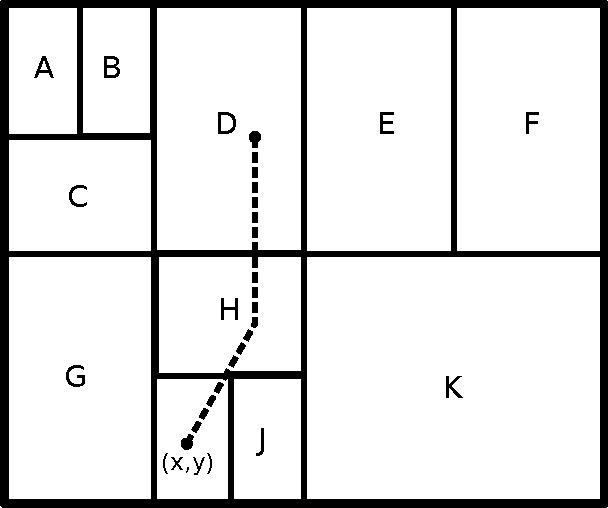
\includegraphics[scale=0.4]{img/algorithms/landmark_binning}
% \caption{Example 2D coordinate overlay and a sample routing path from node D to
% (x,y).}
% \label{fig:landmark_binning}
% \end{figure*}

Landmark Binning \cite{RHMKS2002} is an approach to partition close
by nodes into bins based on their distance to well known anchor nodes across the
Internet.%, as shown in Figure~\ref{fig:landmark_binning}.
In order to detect locality, nodes use network latency (i.e. RTT) as a
measurement technique. The network latency, even though not always accurate, is
selected in this work due to its non-intrusive, transparent and easy to apply
behavior. In order for the binning to work, a few anchor servers with known
physical locations need to be installed in strategic positions accross the the
Internet. Authors estimate that a number of 12 such servers can prove sufficient
for this. Every newly arriving node measures its distance from these landmarks
and unilaterally decides to join a specific bin based on these results.
Specifically, the node measures its round-trip time to each of the landmarks and
orders the values in a decreasing order. The ordering represents a \emph{bin},
in the sense of close-by nodes having the same landmark ordering and hence
belong to the same bin. This means that a landmark system consisting of $m$ such
nodes results in $m!$ potential different bins.The operation of the method is
independent of the model incorporated by the overlay network and thus it can be
applied with no significant changes to both structured and unstructured P2P
systems. \cite{RHMKS2002} has the detailed description of such algorithm for
both architectures. Landmark binning is also considered as a good candidate for
content distribution networks in particular. The major disadvantage of landmark
binning is to install and maintain landmark servers on different autonomous
systems, all over the world. A typical P2P network usually has a couple of
million nodes connected at any given time, thus rendering landmark servers an
important parameter when designing for large scales.  The authors claim that
latency estimation does not drain much from the network resources but in case
scalability problems arise, they claim the solution is replacing single landmark
servers with clusters of servers within the same physical area. However, this
approach does not reduce the possibility of excessive network traffic flow
through these landmark servers. One other possible problem is the incorrect
binning caused by the use of inaccurate methods for delay measurement
(latency is not proven to be a safe way to estimate distance).

%The algorithm can be considered scalable, as nodes need only compute distances
% to a small number of predefined nodes and thus without exchanging any
%information.
%To answer the question as to whether the algorithm actually contributes
% positively to the construction of an enhanced overlay, the paper defines the
%\emph{gain ratio} as the factor by which the latency reduces when someone
%communicates with a random node from the same bin than with one not in the bin.
%This is implemented with an inter-bin to an intra-bin latency ratio.


%
% TODO: LANDMARK BINNING FOR UNSTRUCTURED OVERLAYS
%
%For unstructured overlays the paper assumes \emph{a set of $n$ nodes where each
% node picks any $k$ neighbor nodes so that the average routing latency on the
%resultant overlay is low (assuming shortest path routing)}. According to the
%proposed heuristic algorithm called \emph{BinShort-Long}, a node picks its
%neighbors by choosing its $\frac{k}{2}$ closest\footnote{If the node's bin is
%not large enough for it to pick these $\frac{k}{2}$ neighbors, it picks the
%required nodes from the bin that matches the most in terms of landmark
%ordering.} ones (named \emph{short links}), using the \emph{binning} scheme and
%the rest $\frac{k}{2}$ randomly (\emph{long links}). The former set produces
%well-connected \emph{pockets} of nearby nodes while the later preserves the
%connectivity of the graph, both yielding a proximity factor of $\alpha = 0.5$
%in an attempt to preserve the beneficial properties of unstructured
%topologies\cite{merugu_str2unstr_2003}.

%
% TODO: SOME DISCUSSION
%
%A potential bottleneck could be the extra load that this
%``ping''-like scheme imposes to the landmarks, especially when we need instant
%reaction from our topology when dealing with the dynamic nature of the p2p
%networks.
%
%One disadvantage of this landmark scheme is related to the additional burden
% imposed to the landmark sites. The authors claim though that the algorithm
%requires so little work by the landmarks (maybe just echo to ping messages)
%that could in effect, act as ``unsuspecting participants''. Even if this is the
%case, the fact that it is not fully distributed, renders the protocol's
%scalability directly vulnerable to any system size increase as well as
%suitable for highly dynamic networks such as ad-hoc networks. Moreover, fixed
%points in a network are inherently more exposed to malicious attacks. The most
%significant downside of the algorithm though is that it can lead to an
%extremely uneven overlay ID distribution causing load unbalances and hot spots.
%Lastly, the scheme is coarse grained when it comes to distinguishing relatively
%close nodes\footnote{In the worst case, all nodes could ve clustered into a
%single bin.}.
%

\begin{center}
\begin{tabular}{ccc}
\emph{Efficiency} & \emph{Overhead} & \emph{Scalability} \\
\hline
% The technique is coarse grained thus doesn't achieve optimal results
% (especially in small networks)
medium &
% The overhead is confined to the communication of a node with, most probably,
% 12 landmark servers at most.
low &
% The introduction of landmark servers renders the approach not fully
% decentralized, thus preventing it from scaling smoothly. Communicating
% and overloading landmark servers in high-churn systems is another scalability
% concern.
low
\end{tabular}
\end{center}

%%%%%%%%%%%%%%%%%%%%%%%%%%%%%%%%%%%%%%%%%%%%%%%%%%%%%%%%%%%%%%%%%%%%%%%%%%%%%%%%
\subsubsection{mOverlay}
\emph{mOverlay} \cite{ZZZSZ2004} tries to addresses the scalability issues that
might be imposed to networks (i.e. load unbalance) when using static landmark
servers by introducing dynamic landmarks. Zhang et al. introduce the notion of a
\emph{group} which is a set of peers considered close to each other with respect
to any position in the underlying network, proximity being defined by some
user-defined cost metric like RTT, latency or something else. mOverlay is
considered a clustering approach since it tries to recreate small-world-like
properties to the overlay network by creating a two-level hierarchical
structure, where on the top level we have connections between groups while on
the bottom we have connections between peers inside groups. Finding the correct
closest group is the most important part of the overlay construction. Nodes are
grouped based on their distance to the groups already in the network, rendering
the later (dynamic) landmarks for the process. The authors formally prove
that any new node can reach its group by exchanging at most $O(logN)$ messages
within the network. Finally mOverlay also considers a second important function
in its protocol which is the constant maintenance of the overlay.

%
%\paragraph{Locating process} A new coming host, $Q$, first connects to a
%globally known host cache called the \emph{rendezvous point (RP)} in order to
%retrieve the starting point in the overlay, say $A$ in group $1$. Host $Q$
%then, measures its distance to host $A$. At the same time, the later, sends
%information about the neighbor groups of group $1$ back to host $Q$. This list
%is called \emph{candidate group list}, and the new coming host sequentially
%measures its distance to each of them in seek for the closest one. If the
%\emph{grouping criterion} is met, host $Q$ belongs to group $1$. If not, a boot
%host from the closest group is found and the algorithm is re-run until the
%criterion is met or after a predefined number of repetitions. In the later
%case, $Q$ creates a new group comprising itself only. The above protocol does
%not favor hot-spots as it spreads the probability of visiting a group across
%the whole overlay and limits the overhead in the level of $O \left ( log N
%\right )$.
%
%\paragraph{General overlay operations} A set of additional protocols, are also
% introduced, similar to those found in traditional unstructured networks, but
%modified focusing on scalability and robustness. For example a protocol for
%\emph{group formation} is introduced that exploits the inherent characteristic
%of proximity, in the overlay, in order to efficiently detect the neighboring
%groups of a newly formated group from the set of adjacent groups of its closest
%neighbor. Additionally, during \emph{group joining} the corresponding protocol
%denotes the exchange of important information for group maintenance. This can
%be further improved by \emph{information sharing} between nodes of the same
%group, functionality handled by a dedicated flood-like protocol\footnote{Since
%nodes that belong to the same group are physically close this can be achieved
%at a minimum price.}. Moreover, another set of distributed protocols handle the
%\emph{information update}. The information that needs update, in the proposed
%architecture, is
%\begin{inparaenum}[\itshape i\upshape)]
%  \item the host cache, when a new node joins, and
%  \item the neighbors of groups, when a close-by group is generated.
%\end{inparaenum}
%Finally, in case of \emph{host failure} or \emph{host departure} the system is
% able to maintain its stability since there are defined operations for
%periodical host cache update and group leader selection if one leaves or dies.
%

\begin{center}
\begin{tabular}{ccc}
\emph{Efficiency} & \emph{Overhead} & \emph{Scalability} \\
\hline
% The technique is coarse grained thus doesn't achieve optimal results
% (especially in small networks)
medium &
% The algorithm is iterative through the available groups. At each group
% probing of a candidate list must be performed. This process is done at
% bootstrapping time so the overhead increases in high-churn systems
medium &
% The introduction of dynamic landmark servers renders this approach much more
% scalable than the traditional static landmarking techniques 
medium
\end{tabular}
\end{center}

%%%%%%%%%%%%%%%%%%%%%%%%%%%%%%%%%%%%%%%%%%%%%%%%%%%%%%%%%%%%%%%%%%%%%%%%%%%%%%%%
%%%%%%%%%%%%%%%%%%%%%%%%%%%%%%%%%%%%%%%%%%%%%%%%%%%%%%%%%%%%%%%%%%%%%%%%%%%%%%%%
\subsection{Discussion on the Algorithms for Unstructured Architectures}
%%%%%%%%%%%%%%%%%%%%%%%%%%%%%%%%%%%%%%%%%%%%%%%%%%%%%%%%%%%%%%%%%%%%%%%%%%%%%%%%
%%%%%%%%%%%%%%%%%%%%%%%%%%%%%%%%%%%%%%%%%%%%%%%%%%%%%%%%%%%%%%%%%%%%%%%%%%%%%%%%

% The introduction of landmark servers renders the approach not fully
% decentralized, thus preventing it from scaling smoothly. Communicating
% and overloading landmark servers in high-churn systems is another scalability
% concern.

In this section we introduced the topology mismatching problem from the
perspective of decentralized unstructured architectures and we visited a series
of algorithms that have been proposed in the literature to tackle its negative
influence to networks' performance. Even though, at first glance, the algorithms
seem to do things their own way actually we can distinguish four main
methodologies that are being utilized in order for every algorithm to achieve
its intended result. These methodologies are:
\begin{enumerate}[\itshape i\upshape)]
  \item topology adaptation
  \item forwarding optimization
  \item caching and replication, and
  \item landmarking
\end{enumerate}

Table~\ref{unstructured:table} offers a summarized overview of the algorithms
we saw earlier in the section and tracks down the aforementioned methodologies
each of them incorporates along with their highlights and a rough estimation of
positive and negative aspects of their implementation.

%%%%%%%%%%%%%%%%%%%%%%%%%%%%%%%%%%%%%%%%%%%%%%%%%%%%%%%%%%%%%%%%%%%%%%%%%%%%%%%%
\subsubsection{Topology adaptation}
\begin{figure}[ht]
\centering
\subfigure[Inefficient overlay topology.] {
  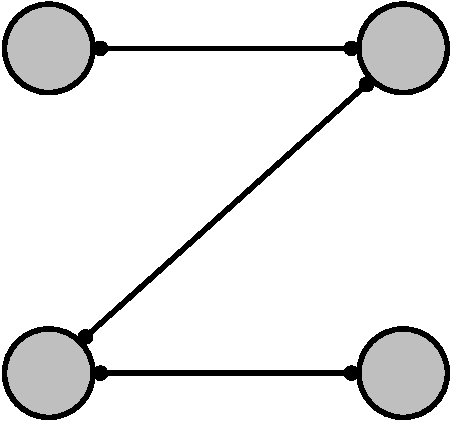
\includegraphics[scale=0.4]{img/pdf/topology-adaptation-before.pdf}
  \label{figure:topology-adaptation:before}
}\qquad\qquad
\subfigure[Efficient overlay topology after adaptation.] {
  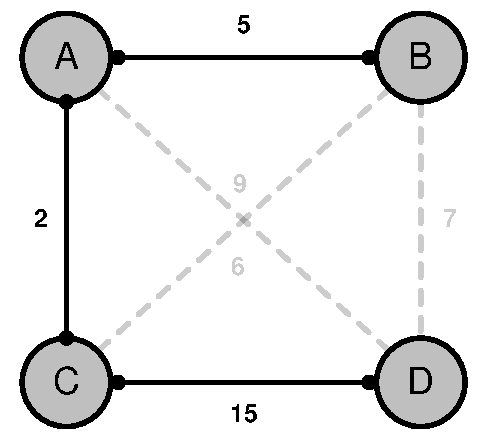
\includegraphics[scale=0.4]{img/pdf/topology-adaptation-after.pdf}
  \label{figure:topology-adaptation:after}
}
\caption{A simple example of how an overlay topology can be adapted.}
\label{figure:topology-adaptation}
\end{figure}

The topology adaptation based protocols modify the topology of the P2P network
using various techniques. The two commonly used approaches that can
back such feature and were investigated in this section are creating
\emph{spanning tree}s using connection graphs, and creating \emph{clusters} of
physically close nodes.

Narada and subsequent algorithms like AOTO, LTM, SBO, try to solve the problem
by building a richer connected graph and forming minimum spanning trees over
this graph that can efficiently route messages among peers. Even though spanning
trees provide efficient query performance, their maintenance costs can be
proven a real blocker. That is why the original Narada algorithm did not have
any real topology adaptation mechanism meaning that it was designed for small
groups (therefore not scalable). Algorithms like AOTO, LTM or SBO try to
overcome these obstacles with clever tricks like forming minimum spanning trees
for the two-hop neighbors ($N^2$) of each node, partitioning the graph into two
random groups where each group is responsible of different tasks, or performing
local optimizations dynamically on the overlay graph. The advantage of building
minimum spanning trees is that they maintain the connectivity on the network in
an efficient manner, while still preserving the overall search scope. However,
their construction and the update costs, especially in dynamic, high-churn
environments, cause large additional traffic overhead to the underlying
network \cite{CRZ2000,CRSZ2001,CRSZ2002}.

The cluster based approaches, on the other hand, select to link physically
closer nodes with each other. T2MC, for example, uses trace-route logs and DDNO
uses domain names to cluster close by nodes. Unfortunately, commonly used
methods for proximity detection across Internet do not always return
reliable results, therefore mapping accuracy is not guaranteed. Moreover,
trace-route, is a heavy-weight utility to be frequently used on the
network, let alone the fact that many network equipment vendors do not allow
trace-route calls at all. The most problematic aspect of clustering, though, is
its nature per se. Limited connectivity among the various local domains can
significantly shrink the search scope, negatively affecting the query response
time the P2P end-user experiences. Of course, techniques that try to round up
such edges and balance the efficiency of the clustering approach with improved
connectivity, have also been proposed, like DDNO, which attempts to address this
limitation by forcing half of each node's connections to be with other, randomly
selected, nodes over the network.

Concluding, topology adaptation ultimately targets on the reduction of the
average cost of the paths from one node to another. This way someone can deduce
that the overlay network is better fit on top of the physical, underlying one.
This deduction is fair in the general case but not always. For example an
adaptive algorithm can exchange a slow edge in the overlay with a faster one
thus reducing the average latency of the network communication. The pitfall here
is that this new virtual link can traverse a fast Autonomous System -to-
Autonomous System link meaning that even though is reduced message
round-trip-time, it has more cost in terms of communication network economics
and management.

% These approaches include creating spanning trees using
%connection graphs, creating cluster of physically close nodes, or using latency
%information to detect proximity. The brief description of each category is
%presented below:
%
%  \begin{itemize}
%    \item \emph{Spanning tree based}. These approaches construct of a rich
%    graph  based on the network connections and build minimum spanning tree
%    on the graphs, causing large traffic overhead to the system
%    \cite{chu_esm_2000,chu_esm_2002}.
%
%    \item \emph{Cluster based}. These approaches select to link physically
%    closer nodes with each other, therefore shrink the search scope
%    significantly while mapping accuracy is not always guaranteed.
%
%    \item \emph{Minimum latency first}. Use of latency as a metric to calculate
%    distance among peers. They require global latency information
%    ``landmarks''\footnote{Measuring latency between peers and stable Internet
%    servers.}.
%
%  \end{itemize}

%%%%%%%%%%%%%%%%%%%%%%%%%%%%%%%%%%%%%%%%%%%%%%%%%%%%%%%%%%%%%%%%%%%%%%%%%%%%%%%%
\subsubsection{Forwarding optimization}

\begin{figure}[ht]
\centering
\subfigure[Typical blind flooding.] {
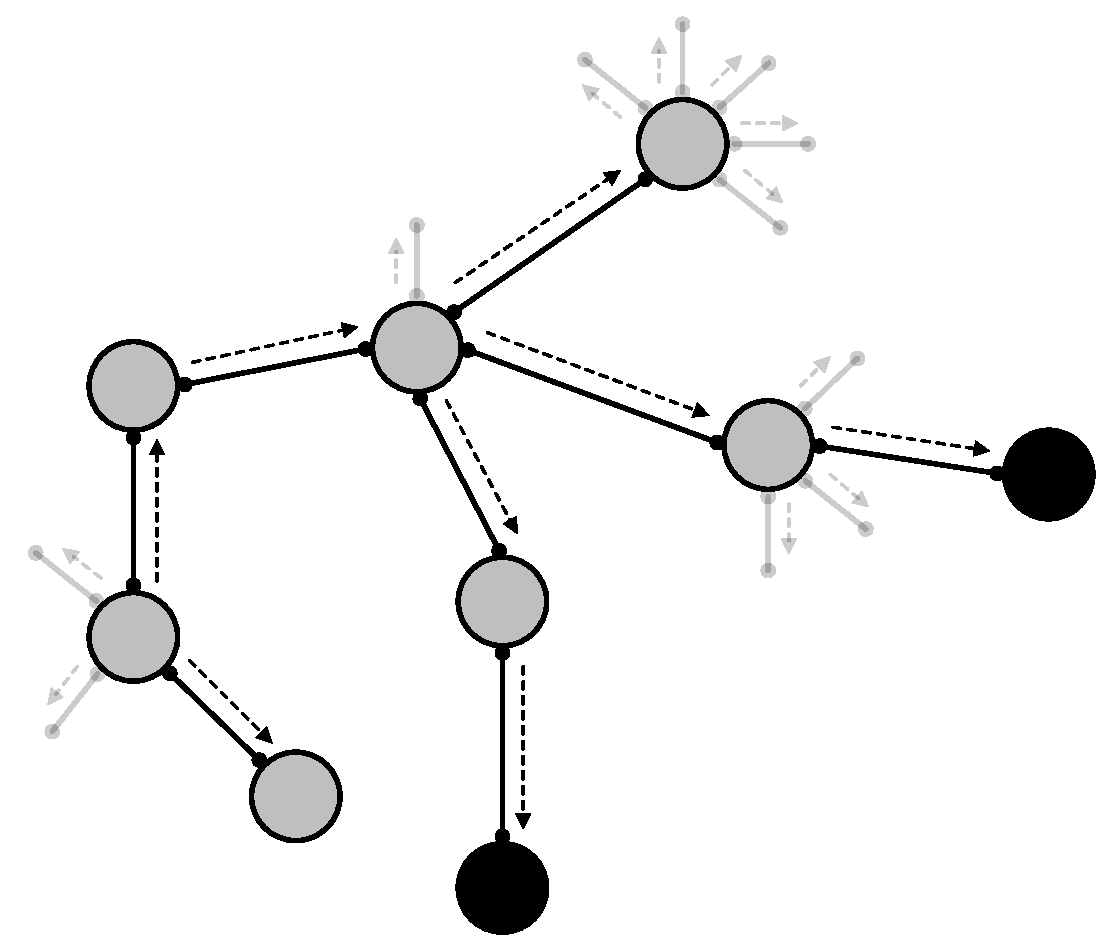
\includegraphics[scale=0.25]{img/pdf/forwarding-optimization-before.pdf}
  \label{figure:forwarding-optimisation:before}
}\qquad\qquad
\subfigure[A node can decide where to forward the messages.] {
  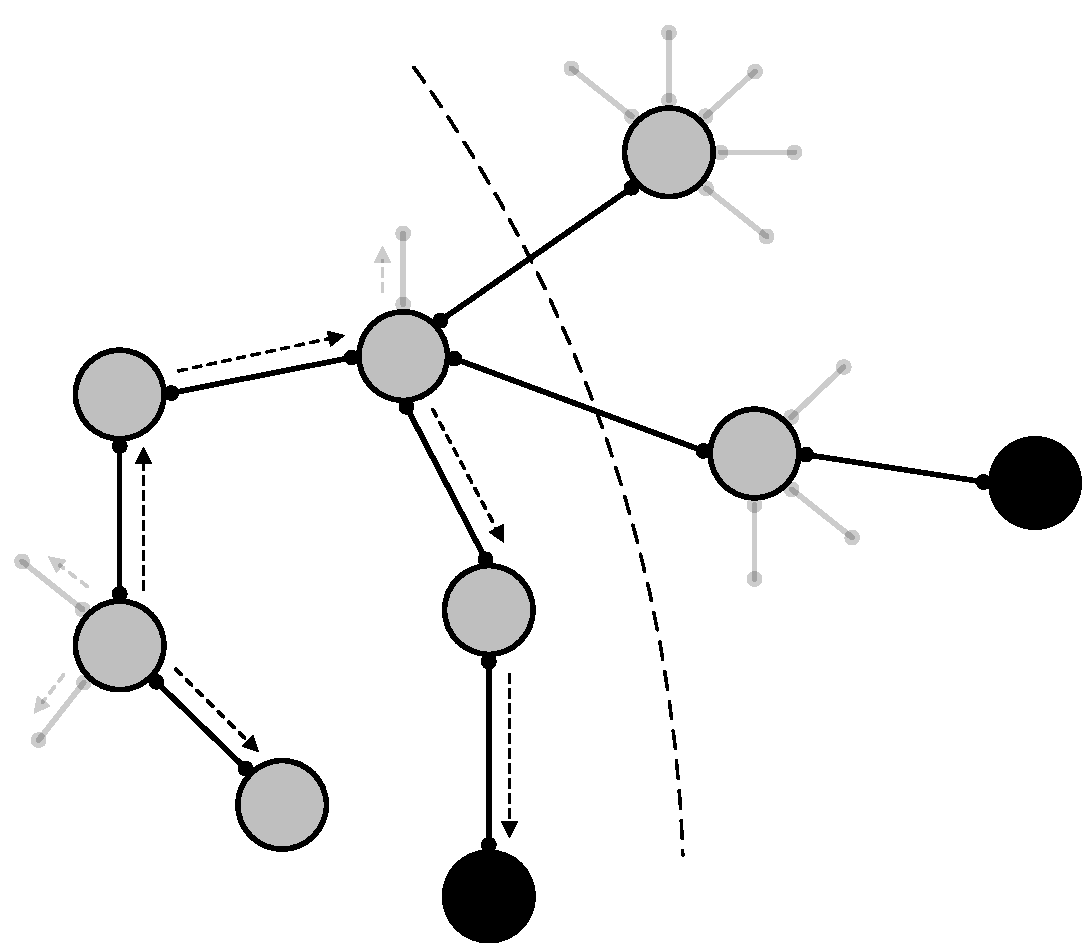
\includegraphics[scale=0.25]{img/pdf/forwarding-optimization-after.pdf}
  \label{figure:forwarding-optimisation:after}
}
\caption{Forwarding optimization in constraining message flooding.}
\label{figure:forwarding-optimisation}
\end{figure}

% Researchers initially started considering alternatives for services who
% implement one-to-many communication schemes, like IP multi-cast, on the
% application layer (i.e. Narada). Application level multi-cast protocols
% are generic protocols that can be applied to both P2P file sharing systems,
% as well as content distribution networks. Application layer multi-cast,
however,
% is not as efficient as the one enabled by IP and still struggles to ease the
% difficulties imposed by the topology mismatch problem.

Forwarding optimization can reduce the emitted messages flooding the overlay and
as a consequence the overall burden, network resources have to handle. In the
first realization of the Gnutella protocol, each query request received by a
peer, was then forwarded to all of its neighbors. This was the source of
unnecessary, sometimes redundant traffic. Forwarding-optimization-based
approaches, propose intelligent forwarding link selection for a message's next
hop across the routing path. The selection criteria vary depending on the
algorithm, but they mainly use one or more statistical heuristics. These can
span from some obvious ones, like the latency of the link between the nodes or
the exposure of specific features, such as high processing bandwidth, high
capacity, or low latency, to more sophisticated alternatives that may even take
into account application level requirements such as the reliability or
friendship. Figure~\ref{figure:forwarding-optimisation} shows a simple example
of how forwarding optimization can work.
Sub-figure~\ref{figure:forwarding-optimisation:before} shows an algorithm that
floods the entire network for search of an object the existence of which is
denoted by black nodes. Alternatively, a node can decide to forward its
messages not to every output link but to a specific or subset of its output
links. In Sub-figure~\ref{figure:forwarding-optimisation:after}, the node in the
middle, does not flood its neighbors. Instead it picks one of them. The dashed
line on the right, shows that, for this routing process, the algorithm has
rendered two potential forwarding paths as inefficient (e.g., the target nodes
show overloading signs). These approaches have the advantage of enhancing the
search responsiveness and reducing the aggregate resource usage of the physical
network. On the other hand, they suffer from drastic reduction of the search
scope (in Sub-figure~\ref{figure:forwarding-optimisation:after} the object on
the far right is not reached) thus limiting the scalability of the whole
network. Moreover they don't actually address the problem of topology mismatch
since they don't give any guarantees that overlay and underlying topologies are
aligned with each other let alone quantify the mismatch and try to alleviate.
Like all other approaches, forwarding based methods are commonly applied in
conjunction with other to improve the quality of the P2P systems.

%Expanding the search scope, on the other hand, is no easy task
%because the overhead of forming multi-cast trees is proportional to the
%multi-cast group size.
%forwarding based schemes do not consider dynamic joining
%and leaving of peers so they do not scale well on dynamic environments.


%%%%%%%%%%%%%%%%%%%%%%%%%%%%%%%%%%%%%%%%%%%%%%%%%%%%%%%%%%%%%%%%%%%%%%%%%%%%%%%%
\subsubsection{Caching and replication}

\begin{figure}[ht]
\centering
\subfigure[Indexing can reduce the cost of the last hop.] {
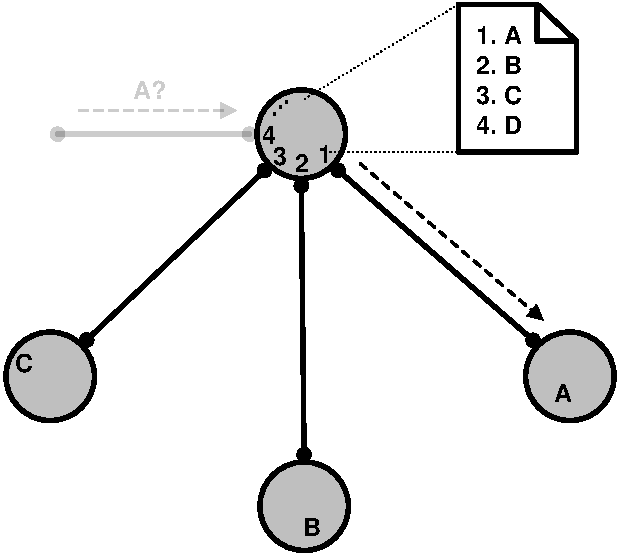
\includegraphics[scale=0.3]{img/pdf/replication-index.pdf}
  \label{figure:replication:index}
}\qquad\qquad
\subfigure[Data replication along the path of a successful query.] {
  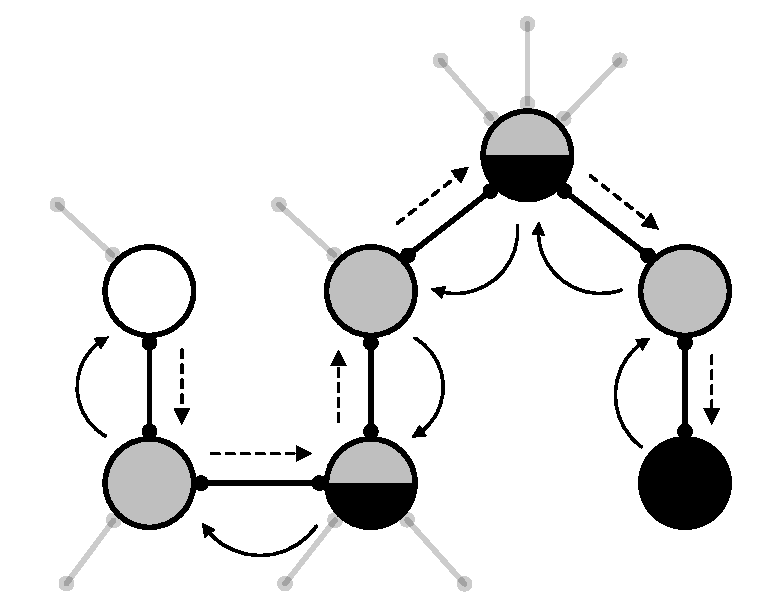
\includegraphics[scale=0.3]{img/pdf/replication-data.pdf}
  \label{figure:replication:data}
}
\caption{Index and data replication strategies.}
\label{figure:replication}
\end{figure}

Caching is a widely used technique to exploit locality and minimize redundant
transfer of data, previously successfully adopted by web and file server
application environments. Since peers in a P2P system also operate as servers,
it is intuitively expected that P2P file sharing systems can also benefit from
caching in improving performance and reducing overall resource usage. However,
the design of caches in this context is non-trivial compared to the web-based
caching. Due to the fact that each node can act as both a server and a client,
two important issues have to be considered at design time. First, the lifetime
of a query is short, as the nodes join and leave frequently. Second, the result
of a single query string is not always the same, as it is dependent on the
source of the query, the TTL value set for the messages, the current
interconnection of peers and the high volatility of the environment. So, in
order to develop a successful caching system for a P2P architecture, these
parameters also have to be considered. P2P caching/replication can be applied
on two different levels, namely caching indices or pointers to data (see
Sub-figure~\ref{figure:replication:index}) or caching the data itself (see
Sub-figure~\ref{figure:replication:data}). Successful implementations have
already been developed in some commercial P2P systems, like KazaA, which uses
caching of indices on its super-peer level. Unfortunately, even though the
state of the art in P2P algorithms using caching methods reduce the resource
usage of the network, they also fail to consistently address typical problems
of a topologically mismatched environment such as duplication of messages.

%\subsection{Cache Based}
%
%Caching based protocols are effectively used to reduce traffic costs and
%response
%times. The caching policy varies depending on the way protocol handles the
%index and the
%content. Centralized P2P systems
%use central index servers, while local caching systems, such as KazaA, use
%super peers
%to cache indices in a distributed way. Content caching is also possible in P2P
%systems, where nodes cache the forwarded content for further retrievals.
%Although caching has the above mentioned advantages,  duplication
%of messages still exist, which limits the scalability of these approaches.
%Therefore, cache based approaches are analyzed in the following categories:
%  \begin{itemize}
%    \item \emph{data index caching},
%    \item \emph{content index caching},
%    \item \emph{centralized}, and
%    \item \emph{local}.
%  \end{itemize}

%%%%%%%%%%%%%%%%%%%%%%%%%%%%%%%%%%%%%%%%%%%%%%%%%%%%%%%%%%%%%%%%%%%%%%%%%%%%%%%%
\subsubsection{Landmarking}\label{sec:landmark}

\begin{figure}[ht]
\centering
  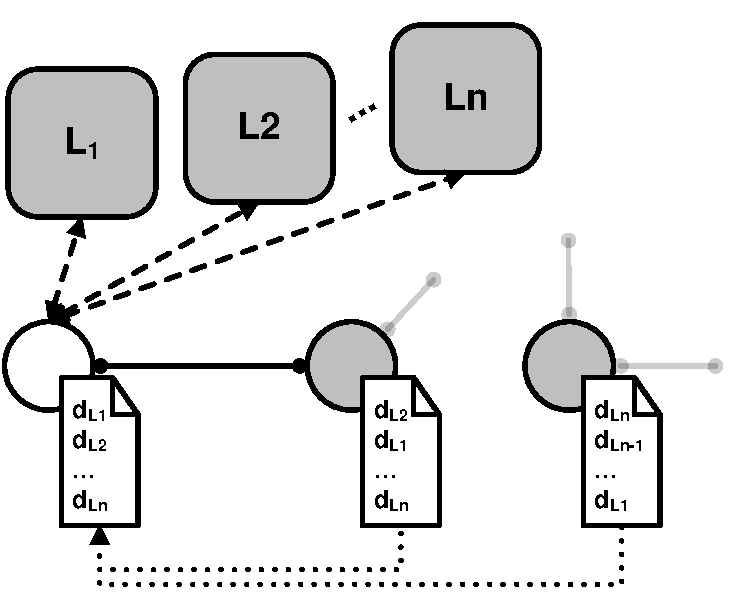
\includegraphics[scale=0.4]{img/pdf/landmarking.pdf}
\caption{Landmark binning during node bootstrap.}
\label{figure:landmarking}
\end{figure}

In landmark-based algorithms, nodes use network delay (e.g. RTT) as a
distance measurement method to position themselves with respect to ``a priori''
known servers (the landmark servers) on the Internet. Landmark servers are used
by nodes to estimate their positions based on the intuitive assumption that
nodes
with similar distances to a set of landmarks, are physically close to each
other, as well, over the network. In Figure~\ref{figure:landmarking} the newly
arriving peer, measures its distance to an array of landmark point denoted as
$Ln$ and and makes a sorted list of the peers, say in increasing order. Then in
order to choose the already participating peers with which to connect to,
compares its list to the list of the potential neighbor. Peers with similar
measured distances to the these landmark points is very likely to be close to
each other as well.

Landmark based protocols has four important drawbacks. Firstly the network
delay is not a reliable distance estimation method. For example, based on the
load on the network the delay to certain nodes or networks can change from time
to time, which will eventually affect the distance measurements and wrong
measurements will lead to wrong estimated positions for the nodes, or incorrect
and non optimal clusterings of the nodes. Secondly, relying on predefined nodes
make the whole paradigm not fully distributed and the landmark system prone to
become a single point of failure. Moreover, the third drawback of using
landmark servers is the cost of installing and maintaining this kind of
infrastructure across the whole Internet and for all the different autonomous
system domains. As popular P2P file sharing applications usually have millions
of peers connected at any time, it is not false to assume that the network costs
of maintaining these landmark servers will be quite high. A possible solution to
the scalability problem of the static landmark servers is to use ordinary nodes
as dynamic landmarks once they estimate their own positions. Even though this
approach scales much better than static landmark servers, still the measurement
accuracy problem affects the overall performance of the system. Moreover,it can
be characterized as a rather coarse-grained approximation, therefore not
particularly well suited for detecting the correct positions of nodes within
close distance to each other.

%%%%%%%%%%%%%%%%%%%%%%%%%%%%%%%%%%%%%%%%%%%%%%%%%%%%%%%%%%%%%%%%%%%%%%%%%%%%%%%%
%\renewcommand\arraystretch{1.9}% (MyValue=1.0 is for standard)

\begin{landscape}
%\begin{figure}[h!]
\hspace{-3ex}
\begin{center}
\footnotesize
%\begin{tabular}{
\begin{longtable}{
|m{2cm}
|m{1cm}
|m{1cm}
|m{1cm}
|m{1cm}
|m{3cm}
|m{5cm}
|
}
% |>{\columncolor[gray]{.7}}m{0.1\columnwidth}
% |>{\columncolor[gray]{.9}}m{0.1\columnwidth}
% |>{\columncolor[gray]{.8}}m{0.1\columnwidth}
% |>{\columncolor[gray]{.9}}m{0.1\columnwidth}
% |>{\columncolor[gray]{.9}}m{0.1\columnwidth}
% |>{\columncolor[gray]{.8}}m{0.1\columnwidth}
% |>{\columncolor[gray]{.9}}m{0.1\columnwidth}
% |}
\caption[Summary table for unstructured algorithms]{Summary table for unstructured algorithms.} \label{unstructured:table} \\
\hline
%%%%%%%%%%%%%%%%%%%%%%%%%%%%%%%%%%%%%%%%%%%%%%%%%%%%%%%%%%%%%%%%%%%%%%%%%%%%%%%%
% first head
\rowcolor[gray]{.5}
\textbf{Algorithm / Paper} &
\textbf{Topology Adaptation} &
\textbf{Forwarding Optimization} &
\textbf{Caching / Replication} &
\textbf{Landmarking} &
\textbf{Highlights} &
\textbf{Pros / Cons}\\
\hline
\endfirsthead
%%%%%%%%%%%%%%%%%%%%%%%%%%%%%%%%%%%%%%%%%%%%%%%%%%%%%%%%%%%%%%%%%%%%%%%%%%%%%%%%
% subsequent heads
\multicolumn{7}{c}%
{\tablename\ \thetable\ -- \textit{Continued from previous page}} \\
\hline
\rowcolor[gray]{.5}
\textbf{Algorithm / Paper} &
\textbf{Topology Adaptation} &
\textbf{Forwarding Optimization} &
\textbf{Caching / Replication} &
\textbf{Landmarking} &
\textbf{Highlights} &
\textbf{Pros / Cons}\\
\hline
\endhead
%%%%%%%%%%%%%%%%%%%%%%%%%%%%%%%%%%%%%%%%%%%%%%%%%%%%%%%%%%%%%%%%%%%%%%%%%%%%%%%%
% foot
\hline \multicolumn{7}{r}{\textit{Continued on next page}} \\
\endfoot
%%%%%%%%%%%%%%%%%%%%%%%%%%%%%%%%%%%%%%%%%%%%%%%%%%%%%%%%%%%%%%%%%%%%%%%%%%%%%%%%
% last foot
\hline
\endlastfoot
%%%%%%%%%%%%%%%%%%%%%%%%%%%%%%%%%%%%%%%%%%%%%%%%%%%%%%%%%%%%%%%%%%%%%%%%%%%%%%%%
% data
\textbf{\cite{YG-M2002}} &
{\large \Square} &
{\large \CheckedBox} &
{\large \CheckedBox} &
{\large \Square} &
\begin{tabular}[l]{m{3cm}}
Iterative Deepening (ID).\\
Directed BFS (DBFS).\\
Local Indices (LI).
\end{tabular} &
\begin{tabular}[l]{m{5cm}}
+ ID reduces the messages especially in upper levels of the tree.\\
%+ DBFS ??????\\
+ LI reduces aggregate bandwidth usage and improves query efficiency.\\
-- ID needs evaluation time between iterations.\\
-- DBFS uses heuristics so it depends on their efficient choice.\\
-- LI add index update overhead which might be heavy process especially in high-churn systems.
\end{tabular}
\\
\hline
%%%%%%%%%%%%%%%%%%%%%%%%%%%%%%%%%%%%%%%%%%%%%%%%%%%%%%%%%%%%%%%%%%%%%%%%%%%%%%%%
\textbf{DAPS \cite{ZL2005}} &
{\large \Square} &
{\large \Square} &
{\large \Square} &
{\large \Square} &
\begin{tabular}[l]{m{3cm}}
Clustered routing tables based on delay.\\
Pruning flood, an iterative deepening and multiple BFS approach with a pruning
boundary.
\end{tabular} &
+ It is a system between structured and unstructured.
\\
\hline
%%%%%%%%%%%%%%%%%%%%%%%%%%%%%%%%%%%%%%%%%%%%%%%%%%%%%%%%%%%%%%%%%%%%%%%%%%%%%%%%
\textbf{Gia \cite{CRBLS2003}} &
{\large \CheckedBox} &
{\large \CheckedBox} &
{\large \CheckedBox} &
{\large \Square} &
\begin{tabular}{m{3cm}}
Random Walks (RW).
\end{tabular} &
\begin{tabular}[l]{m{5cm}}
+ RWs issue one copy of the query thus not flooding the whole network.\\
-- RWs can reduce search scope.\\
\end{tabular}
\\
\hline
%%%%%%%%%%%%%%%%%%%%%%%%%%%%%%%%%%%%%%%%%%%%%%%%%%%%%%%%%%%%%%%%%%%%%%%%%%%%%%%%
\textbf{DCMP \cite{ZKB2008}} &
{\large \CheckedBox} &
{\large \Square} &
{\large \Square} &
{\large \Square} &
\begin{tabular}{m{3cm}}
Cycle detection.
\end{tabular} &
\begin{tabular}[l]{m{5cm}}
+ Drastically reduces duplicate messages.\\
-- Cannot detect cycles in distance bigger than the TTL value of the IC message.\\
\end{tabular}
\\
\hline
%%%%%%%%%%%%%%%%%%%%%%%%%%%%%%%%%%%%%%%%%%%%%%%%%%%%%%%%%%%%%%%%%%%%%%%%%%%%%%%%
\textbf{\cite{CS2002}} &
{\large \Square} &
{\large \Square} &
{\large \CheckedBox} &
{\large \Square} &
\begin{tabular}[l]{m{3cm}}
Uniform replication.\\
Proportional replication.\\
Square root replication allocation.
\end{tabular} &
\begin{tabular}[l]{m{5cm}}
+ Uniform replication reduces time spend on unsuccessful searches.\\
+ Reduces search time for frequent queries.\\
-- Proportional replication struggles in locating rare objects.
\end{tabular}
\\
\hline
%%%%%%%%%%%%%%%%%%%%%%%%%%%%%%%%%%%%%%%%%%%%%%%%%%%%%%%%%%%%%%%%%%%%%%%%%%%%%%%%
% \textbf{Tracing a large-scale Peer to Peer System: an hour in the life of Gnutella} &
% ? &
% ? &
% ? &
% ? &
% ? &
% ?
% \\
% \hline
%%%%%%%%%%%%%%%%%%%%%%%%%%%%%%%%%%%%%%%%%%%%%%%%%%%%%%%%%%%%%%%%%%%%%%%%%%%%%%%%
\textbf{Narada \cite{CRZ2000}} &
{\large \Square} &
{\large \CheckedBox} &
{\large \Square} &
{\large \Square} &
\begin{tabular}[l]{m{3cm}}
Mess creation.\\
Minimum spanning trees.
\end{tabular} &
\begin{tabular}[l]{m{5cm}}
+ Mess and trees are kept up to date in high churn environments.\\
-- Works well only for small groups of peers.
\end{tabular}
\\
\hline
%%%%%%%%%%%%%%%%%%%%%%%%%%%%%%%%%%%%%%%%%%%%%%%%%%%%%%%%%%%%%%%%%%%%%%%%%%%%%%%%
\textbf{AOTO \cite{LZXN2003}} &
{\large \CheckedBox} &
{\large \CheckedBox} &
{\large \Square} &
{\large \Square} &
\begin{tabular}[l]{m{3cm}}
Minimum spanning trees.\\
Peer proximity heuristic for removing costly links.
\end{tabular} &
\begin{tabular}[l]{m{5cm}}
+ Spanning trees only to immediate neighbors so no flooding and at the same time
no shrinked search scope.\\
+ Selective flooding effectiveness is detached from physical or overlay topologies.\\
+ The more logical neighbors, the more effective selective flooding becomes\\
-- High recalculation costs.\\
-- No sophisticated selection policy for candidate non-flooding peers.
\end{tabular}
\\
\hline
%%%%%%%%%%%%%%%%%%%%%%%%%%%%%%%%%%%%%%%%%%%%%%%%%%%%%%%%%%%%%%%%%%%%%%%%%%%%%%%%
\textbf{ACE \cite{LZXN2004}} &
{\large \CheckedBox} &
{\large \CheckedBox} &
{\large \Square} &
{\large \Square} &
\begin{tabular}[l]{m{3cm}}
Minimum spanning trees.\\
1-hop proximity heuristic.
\end{tabular} &
\begin{tabular}[l]{m{5cm}}
+ No flooding.\\
+ Less overhead compared to AOTO since computation is done within a certain diameter from the source peer.
-- Slow convergence speed.\\
-- Enhanced topology optimization comes to the expence of higher communication/computation overhead.
\end{tabular}
\\
\hline
%%%%%%%%%%%%%%%%%%%%%%%%%%%%%%%%%%%%%%%%%%%%%%%%%%%%%%%%%%%%%%%%%%%%%%%%%%%%%%%%
\textbf{LTM \cite{LLXNZ2004}} &
{\large \CheckedBox} &
{\large \Square} &
{\large \Square} &
{\large \Square} &
\begin{tabular}[l]{m{3cm}}
TTL detector (2-hop distance).\\
Delayed low productive connection cutting.
\end{tabular} &
\begin{tabular}[l]{m{5cm}}
+ Compared to AOTO, ACE and SBO achieves faster convergence speed.\\
-- Creates more overhead than AOTO, ACE and SBO.\\
-- Needs synchronization of peer clocks.\\
-- Does not consider shortcuts created by powerful peers when choosing to disable connections (only uses delay metric).
\end{tabular}
\\
\hline
%%%%%%%%%%%%%%%%%%%%%%%%%%%%%%%%%%%%%%%%%%%%%%%%%%%%%%%%%%%%%%%%%%%%%%%%%%%%%%%%
\textbf{SBO \cite{LXN2004}} &
{\large \CheckedBox} &
{\large \CheckedBox} &
{\large \Square} &
{\large \Square} &
\begin{tabular}{m{3cm}}
Red/white bipartite overlay.
\end{tabular} &
\begin{tabular}[l]{m{5cm}}
+ Efficient in both static and dynamic environments.\\
+ Compared to AOTO incurs half the overhead.\\
-- Needs almost double the steps of LTM to converge (static or dynamic environments).
\end{tabular}
\\
\hline
%%%%%%%%%%%%%%%%%%%%%%%%%%%%%%%%%%%%%%%%%%%%%%%%%%%%%%%%%%%%%%%%%%%%%%%%%%%%%%%%
\textbf{THANCS \cite{LNXE2005}} &
{\large \CheckedBox} &
{\large \CheckedBox} &
{\large \Square} &
{\large \Square} &
\begin{tabular}[l]{m{3cm}}
Local optimum heuristic\\
Piggybacking neighbor distance in queries
\end{tabular} &
\begin{tabular}[l]{m{5cm}}
+ Completely distributed approach.\\
+ Presents trivial overhead compared to the query cost savings.\\
+ Convergent speed faster among AOTO, LTM, SBO.\\
+ Does not shrink the search scope.\\
-- Design cannot be extended to support non-flooding-based systems.
\end{tabular}
\\
\hline
%%%%%%%%%%%%%%%%%%%%%%%%%%%%%%%%%%%%%%%%%%%%%%%%%%%%%%%%%%%%%%%%%%%%%%%%%%%%%%%%
\textbf{HAND \cite{CLZHC2006}} &
{\large \CheckedBox} &
{\large \Square} &
{\large \Square} &
{\large \Square} &
\begin{tabular}{m{3cm}}
Triple-hop adjustment.
\end{tabular} &
\begin{tabular}[l]{m{5cm}}
+ No need for clock sync.\\
+ Fully distributed.\\
+ Low overhead for the triple hop adjustment.\\
+ Applicable to both static and dynamic environments.\\
+ Low query response time.\\
-- Compared to LTM has lower traffic reduction and query response rates.
\end{tabular}
\\
\hline
%%%%%%%%%%%%%%%%%%%%%%%%%%%%%%%%%%%%%%%%%%%%%%%%%%%%%%%%%%%%%%%%%%%%%%%%%%%%%%%%
\textbf{APS \cite{BFLZ2003}} &
{\large \CheckedBox} &
{\large \Square} &
{\large \Square} &
{\large \Square} &
\begin{tabular}{m{3cm}}
machine learning adaptive mechanism.
\end{tabular} &
\begin{tabular}[l]{m{5cm}}
+ Fully dynamic switching decision policy.\\
- Low convergence due to the learning process.
\end{tabular}
\\
\hline
%%%%%%%%%%%%%%%%%%%%%%%%%%%%%%%%%%%%%%%%%%%%%%%%%%%%%%%%%%%%%%%%%%%%%%%%%%%%%%%%
\textbf{ITA \cite{PRFM2009}} &
{\large \CheckedBox} &
{\large \CheckedBox} &
{\large \Square} &
{\large \Square} &
\begin{tabular}[l]{m{3cm}}
Short/long connections.\\
Local flooding.
\end{tabular} &
\begin{tabular}[l]{m{5cm}}
+ Low clustering.\\
+ Large peer coverage.\\
+ Reduced duplication.\\
+ Low or no impact to other mechanisms of unstructured p2p networks (e.g. 1-hop
replication, dynamic querying).
\end{tabular}
\\
\hline
%%%%%%%%%%%%%%%%%%%%%%%%%%%%%%%%%%%%%%%%%%%%%%%%%%%%%%%%%%%%%%%%%%%%%%%%%%%%%%%%
\textbf{EGOIST \cite{SLLBBR2008}} &
{\large \CheckedBox} &
{\large \Square} &
{\large \Square} &
{\large \Square} &
\begin{tabular}{m{3cm}}
Selfish shortest path routing
\end{tabular} &
\begin{tabular}{m{3cm}}
-- constructs a global view of the network
\end{tabular}
\\
\hline
%%%%%%%%%%%%%%%%%%%%%%%%%%%%%%%%%%%%%%%%%%%%%%%%%%%%%%%%%%%%%%%%%%%%%%%%%%%%%%%%
\textbf{BNS \cite{BCCMSBZ2006}} &
{\large \CheckedBox} &
{\large \Square} &
{\large \CheckedBox} &
{\large \Square} &
\begin{tabular}[l]{m{3cm}}
ISP clustering (tracker-side or ISP-side detection).\\
Bandwidth throttling.\\
Caching.
\end{tabular} &
\begin{tabular}[l]{m{5cm}}
+ Localizes traffic within an ISP.\\
+ Preserves the efficiency of BitTorrent protocol.\\
-- Needs ISPs to either provide information or infrastructure changes.\\
-- Locality-based approaches do not treat fair all peers.
\end{tabular}
\\
\hline
%%%%%%%%%%%%%%%%%%%%%%%%%%%%%%%%%%%%%%%%%%%%%%%%%%%%%%%%%%%%%%%%%%%%%%%%%%%%%%%%
\textbf{Ono \cite{CB2008}} &
{\large \CheckedBox} &
{\large \Square} &
{\large \Square} &
{\large \CheckedBox} &
\begin{tabular}[l]{m{3cm}}
ISP clustering.\\
Landmarking based on existing CDN infrastructure (CDN redirection measurements).
\end{tabular} &
\begin{tabular}[l]{m{5cm}}
+ Needs no ISP cooperation.\\
+ Needs no extra infrastructure.\\
+ Needs no network topology information.\\
-- Locality based approaches do not treat fair all peers.
\end{tabular}
\\
\hline
%%%%%%%%%%%%%%%%%%%%%%%%%%%%%%%%%%%%%%%%%%%%%%%%%%%%%%%%%%%%%%%%%%%%%%%%%%%%%%%%
\textbf{\cite{LCLX2009}} &
{\large \CheckedBox} &
{\large \Square} &
{\large \Square} &
{\large \Square} &
\begin{tabular}{m{3cm}}
AS hop count minimization on neighbor selection, on chocking/unchocking
mechanisms and on next-chunk picking.
\end{tabular} &
\begin{tabular}[l]{m{5cm}}
+ Optimization of the inter-AS traffic.\\
-- Locality based approaches do not treat fair all peers.
\end{tabular}
\\
\hline
%%%%%%%%%%%%%%%%%%%%%%%%%%%%%%%%%%%%%%%%%%%%%%%%%%%%%%%%%%%%%%%%%%%%%%%%%%%%%%%%
\textbf{TopBT \cite{RTLCGZ2010}} &
{\large \CheckedBox} &
{\large \Square} &
{\large \Square} &
{\large \Square} &
\begin{tabular}[l]{m{3cm}}
Peer selection metric that takes both downloading speed and network topology
into account.\\
Applied in multiple places of the BitTorrent protocol (bootstrap, connection
establishment/replacement, unchocking).
\end{tabular} &
\begin{tabular}[l]{m{5cm}}
+ No need for additional infrastructure.\\
+ Enhances both traffic and downloading.\\
-- Needs off-line processing of BGP dumps.
\end{tabular}
\\
\hline
%%%%%%%%%%%%%%%%%%%%%%%%%%%%%%%%%%%%%%%%%%%%%%%%%%%%%%%%%%%%%%%%%%%%%%%%%%%%%%%%
\textbf{UTAPS \cite{LCY2008}} &
{\large \CheckedBox} &
{\large \Square} &
{\large \Square} &
{\large \CheckedBox} &
\begin{tabular}{m{3cm}}
Network tomography to construct a picture for the underlying network.
\end{tabular} &
\begin{tabular}[l]{m{5cm}}
+ Reduced ISP burden.\\
+ Better downloading speeds.\\
-- Small, laboratory-scale evaluation setup.
\end{tabular}
\\
\hline
%%%%%%%%%%%%%%%%%%%%%%%%%%%%%%%%%%%%%%%%%%%%%%%%%%%%%%%%%%%%%%%%%%%%%%%%%%%%%%%%
\textbf{\cite{QLZG2009}} &
{\large \CheckedBox} &
{\large \Square} &
{\large \Square} &
{\large \CheckedBox} &
\begin{tabular}{m{3cm}}
Cluster peers in a swarm into local, intra- and inter-ISP.
\end{tabular} &
\begin{tabular}[l]{m{5cm}}
+ Reduced ISP burden.\\
+ Better downloading speeds.\\
-- Similarly to UTAPS, the evaluation setup was small scale.
\end{tabular}
\\
\hline
%%%%%%%%%%%%%%%%%%%%%%%%%%%%%%%%%%%%%%%%%%%%%%%%%%%%%%%%%%%%%%%%%%%%%%%%%%%%%%%%
\textbf{PROP \cite{QCYCZ2007}} &
{\large \CheckedBox} &
{\large \Square} &
{\large \Square} &
{\large \Square} &
\begin{tabular}{m{3cm}}
Neighbor exchange between peers.
\end{tabular} &
\begin{tabular}[l]{m{5cm}}
+ Cooperation between peers.\\
+ Guarantees the connectivity of the network between exchanges.\\
\end{tabular}
\\
\hline
%%%%%%%%%%%%%%%%%%%%%%%%%%%%%%%%%%%%%%%%%%%%%%%%%%%%%%%%%%%%%%%%%%%%%%%%%%%%%%%%
% \textbf{Resolving the Topology Mismatch Problem in Unstructured Peer-to-Peer Networks} &
% ? &
% ? &
% ? &
% ? &
% ? &
% ?
% \\
% \hline
%%%%%%%%%%%%%%%%%%%%%%%%%%%%%%%%%%%%%%%%%%%%%%%%%%%%%%%%%%%%%%%%%%%%%%%%%%%%%%%%
\textbf{DDNO \cite{Z-YK2005}} &
{\large \CheckedBox} &
{\large \Square} &
{\large \Square} &
{\large \Square} &
\begin{tabular}{m{3cm}}
Domain name topology detection (Split-Hash and dnMatch).
\end{tabular} &
\begin{tabular}[l]{m{5cm}}
+ Can be applied to both fully unstructured and super-peer based architectures.\\
+ Secures connectivity of the network.\\
+ Reduces cost of message exchange.
\end{tabular}
\\
\hline
%%%%%%%%%%%%%%%%%%%%%%%%%%%%%%%%%%%%%%%%%%%%%%%%%%%%%%%%%%%%%%%%%%%%%%%%%%%%%%%%
\textbf{CTAG \cite{ZL2006}} &
{\large \CheckedBox} &
{\large \Square} &
{\large \Square} &
{\large \Square} &
\begin{tabular}{m{3cm}}
Clustering based on longest matching IP segment.
\end{tabular} &
\begin{tabular}{m{5cm}}
+ Focuses on both construction and adaptation.
\end{tabular}
\\
\hline
%%%%%%%%%%%%%%%%%%%%%%%%%%%%%%%%%%%%%%%%%%%%%%%%%%%%%%%%%%%%%%%%%%%%%%%%%%%%%%%%
\textbf{Landmark Binning \cite{RHMKS2002}} &
{\large \CheckedBox} &
{\large \Square} &
{\large \Square} &
{\large \CheckedBox} &
\begin{tabular}{m{3cm}}
Landmark binning.
\end{tabular} &
\begin{tabular}[l]{m{5cm}}
+ It is independent of the overlay model.\\
+ The technique can be considered scalable.\\
-- Uses not so reliable network latency metric (this can lead to load imbalance etc).\\
-- The use of landmark servers renders the technique not fully distributed.\\
-- Excessive traffic flow towards the landmark servers is possible.\\
-- Fixed points in a network are inherently more exposed to malicious attacks.\\
-- Coarse-grained scheme.
\end{tabular}
\\
\hline
%%%%%%%%%%%%%%%%%%%%%%%%%%%%%%%%%%%%%%%%%%%%%%%%%%%%%%%%%%%%%%%%%%%%%%%%%%%%%%%%
\textbf{mOverlay \cite{ZZZSZ2004}} &
{\large \CheckedBox} &
{\large \Square} &
{\large \Square} &
{\large \CheckedBox} &
\begin{tabular}{m{3cm}}
Dynamic landmarks.
\end{tabular} &
\begin{tabular}[l]{m{5cm}}
+ Fully distributed.\\
+ It is independent of the overlay model.\\
-- Coarse-grained scheme.
\end{tabular}
\\
\hline
%%%%%%%%%%%%%%%%%%%%%%%%%%%%%%%%%%%%%%%%%%%%%%%%%%%%%%%%%%%%%%%%%%%%%%%%%%%%%%%%


%\begin{tabular}[l]{@{}}
%+ ID reduces the messages especially in upper levels of the tree\\
%+ DBFS\\
%+ LI reduces aggregate bandwidth usage and improves query efficiency\\
%- ID needs evaluation time between iterations\\
%- DBFS uses heuristics so it depends on their efficient choice\\
%- LI add index update overhead which might be heavy and might not work at all in systems with high churn
%\end{tabular} &


%\textbf{Narada} & \textbf{Overlay optimization
%based}. Creates a mesh (richer connected graph) and builds minimum spanning
%trees on this mesh & & Small and sparse groups \\

%\hline
%\textbf{Gia} & \textbf{Broadcast based} Replaces
%Gnutella flooding with random walk, and introduces KaZaA style super-nodes.
%Uses
%dynamic topology adaptation protocol &
% Gnutella &  Better than Gnutella  \\

%\hline
%\textbf{Adaptive Overlay Topology Optimization} & \textbf{Overlay optimization
%based}. Creates overlay multi-cast tree with Selective Flooding protocol&
%Gnutella &  Better than Gnutella \\

% \hline
% \textbf{Location-aware Topology Matching} &
% \textbf{Overlay Optimization Based}. Uses \textit{TTL2-detector flooding}, \textit{low productive
% connection cutting}, and \textit{source peer probing}. & Gnutella &  Better than Gnutella \\
% 
% \hline
% \textbf{Replication Strategies in Unstructured P2P Networks} &
% \textbf{Cache Based}. Uses uniform, proportional and square root allocation
% strategies to replicate data. & Gnutella &  Better than Gnutella \\
% 
% % \hline
% \textbf{Tracing a large-scale Peer to Peer System: an hour in the life of Gnutella.} &
% \textbf{Cache Based}. Proposes a caching algorithm based on the traces of the Gnutella traffic & Gnutella & Better than Gnutella \\
% 
% \hline
% \textbf{Improving search in P2P networks} &
% \textbf{Broadcast Based}. Uses \textit{iterative deepening}, \textit{directed
% BFS}, and \textit{local indices} to improve efficiency. & Gnutella &  Better than Gnutella \\
% 
% \hline
% \textbf{Distributed Cycle Minimization Protocol} &
% \textbf{Broadcast based} Uses a decentralized cycle elimination protocol  &  &  \\
% 
% \hline
% \textbf{Scalable Bipartite Overlay} &
% \textbf{Overlay optimization based} Uses bipartite partition graph and builds
% local minimum spanning trees  & Gnutella  & Better than Gnutella \\
% 
% \hline
% \textbf{Adaptive Connection Establishment} &
% \textbf{Overlay optimization based} Forms Neighbor Cost Tables, builds local
% minimum spanning trees and perform local optimizations & Adaptive Overlay
% Topology Optimization (AOTO), Gnutella & Better than Gnutella \\

% \hline
% \textbf{Hops Adaptive Neighbor Discovery} &  & &  \\
% 
% \hline
% \textbf{Two-Hop-Away Neighbor Comparison and Selection (THANCS)} &
% \textbf{Overlay optimization based} Uses piggybacking to discover neighbor
% distances and selects neighbors  & Gnutella  & \\

% \hline
% \textbf{mOverlay} &\textbf{Landmark based proximity} Uses dynamic landmarks to find node locality
% & & Due to dynamic landmarks and grouping, more scalable than tree-based or mesh-based protocols \\
% 
% \hline
% \textbf{Distributed Domain Name Order (DDNO)} &
% \textbf{Overlay optimization based} Connects half of the nodes connections to
% the nodes in the same domain and the other half to random nodes, therefore
% supports locality and topological connection  &  & Yes, by using super
% peers \\

% \hline
% \textbf{Peer-exchange Routing Optimization Protocols} & \textbf{Overlay optimization based} Optimizes overlay by the exchange of
% neighbors among peers  & Can work with both decentralized structured and
% unstructured architecture & Yes \\

% \hline
% \textbf{MAY OMIT - I CHANGED IT TO STRUCTURED SINCE THERE IS A REFERENCE FOR
% DHT (OF COURSE IT MIGHT POSSIBLE TO BE APPLIED TO BOTH. MAYBE NEED TO CHECK) -
% T2MC} &
% \textbf{Overlay optimization based} Uses trace-route results for clustering
% the nodes  & & \\
% 
% \hline
% \textbf{Unnamed-unstructured} &
% \textbf{Overlay optimization based} Minimizes the communication delay and
% maximizes the broadcasting range & & Better than THANCS and mOverlay \\

% \hline
% \textbf{Landmark Binning} & \textbf{Landmark based proximity} Uses network latency to partition
% nodes into bins & Can work with both decentralized structured and unstructured architecture & \\
% 
% \hline
%\end{tabular}
\end{longtable}
\end{center}
\vspace{-2.5ex}
\vspace{-2.5ex}
%\end{figure}
\end{landscape}


%%%%%%%%%%%%%%%%%%%%%%%%%%%%%%%%%%%%%%%%%%%%%%%%%%%%%%%%%%%%%%%%%%%%%%%%%%%%%%%%
%%%%%%%%%%%%%%%%%%%%%%%%%%%%%%%%%%%%%%%%%%%%%%%%%%%%%%%%%%%%%%%%%%%%%%%%%%%%%%%%
%                             UNSTRUCTURED
%%%%%%%%%%%%%%%%%%%%%%%%%%%%%%%%%%%%%%%%%%%%%%%%%%%%%%%%%%%%%%%%%%%%%%%%%%%%%%%%
%%%%%%%%%%%%%%%%%%%%%%%%%%%%%%%%%%%%%%%%%%%%%%%%%%%%%%%%%%%%%%%%%%%%%%%%%%%%%%%%

%\pgfplotsset{width=7cm,compat=newest}

%%%%%%%%%%%%%%%%%%% EFFICIENCY %%%%%%%%%%%%%%%%%%%
\begin{landscape}
\begin{center}
\begin{tikzpicture}
\begin{axis}[
  xbar,
  bar width=7pt,
  xlabel=\emph{Efficiency},
  ylabel=\emph{Algorithm},
  symbolic x coords={low, medium, high},
  symbolic y coords={
    IterativeDeepening,
    DirectedBFS,
    LocalIndices,
    DAPS,
    Gia,
    DCMP,
    UniformReplication,
    ProportionalReplication,
    SqrtReplication,
    %Markatos02,
    Narada,
    AOTO,
    ACE,
    LTM,
    SBO,
    THANCS,
    HAND,
    APS,
    ITA,
    EGOIST,
    BNS,
    Ono,
    LiuEtAl,
    TopBT,
    UTAPS,
    QinEtAl,
    PROP-G,
    PROP-O,
    %hsiao_redblue_2009,
    DDNO,
    CTAG,
    LB,
    mOverlay
  },
  every axis y label/.style=
    {at={(ticklabel cs:0.5)},rotate=90,anchor=near ticklabel},
%   x tick label style={rotate=45,anchor=east},
  xtick=data, ytick=data,
%   ymin=low,ymax=high,ytickmin=low,
  height=\textheight - 0.3cm,
  width=\textwidth,
  enlargelimits=0.05,
  title=\emph{Efficiency} Pictorial Comparison of Unstructured Approaches.
]

\addplot[black,fill=gray!20, postaction={pattern=north east lines}]
table[x=EFFICIENCY,y=ALGORITHM]
{unstructured-plot.dat};

\end{axis}
\end{tikzpicture}
\end{center}
\end{landscape}

%%%%%%%%%%%%%%%%%%% OVERHEAD %%%%%%%%%%%%%%%%%%%
\begin{landscape}
\begin{center}
\begin{tikzpicture}
\begin{axis}[
  xbar,
  bar width=7pt,
  xlabel=\emph{Overhead},
  ylabel=\emph{Algorithm},
  symbolic x coords={low, medium, high},
  symbolic y coords={
    IterativeDeepening,
    DirectedBFS,
    LocalIndices,
    DAPS,
    Gia,
    DCMP,
    UniformReplication,
    ProportionalReplication,
    SqrtReplication,
    %Markatos02,
    Narada,
    AOTO,
    ACE,
    LTM,
    SBO,
    THANCS,
    HAND,
    APS,
    ITA,
    EGOIST,
    BNS,
    Ono,
    LiuEtAl,
    TopBT,
    UTAPS,
    QinEtAl,
    PROP-G,
    PROP-O,
    %hsiao_redblue_2009,
    DDNO,
    CTAG,
    LB,
    mOverlay
  },
  every axis y label/.style=
    {at={(ticklabel cs:0.5)},rotate=90,anchor=near ticklabel},
%   x tick label style={rotate=45,anchor=east},
  xtick=data, ytick=data,
%   ymin=low,ymax=high,ytickmin=low,
  height=\textheight - 0.3cm,
  width=\textwidth,
  enlargelimits=0.05,
  title=\emph{Overhead} Pictorial Comparison of Unstructured Approaches.
]

\addplot[black,fill=gray!20, postaction={pattern=crosshatch}]
table[x=OVERHEAD,y=ALGORITHM]
{unstructured-plot.dat};

\end{axis}
\end{tikzpicture}
\end{center}
\end{landscape}

%%%%%%%%%%%%%%%%%%% SCALABILITY %%%%%%%%%%%%%%%%%%%
\begin{landscape}
\begin{center}
\begin{tikzpicture}
\begin{axis}[
  xbar,
  bar width=7pt,
  xlabel=\emph{Scalability},
  ylabel=\emph{Algorithm},
  symbolic x coords={low, medium, high},
  symbolic y coords={
    IterativeDeepening,
    DirectedBFS,
    LocalIndices,
    DAPS,
    Gia,
    DCMP,
    UniformReplication,
    ProportionalReplication,
    SqrtReplication,
    %Markatos02,
    Narada,
    AOTO,
    ACE,
    LTM,
    SBO,
    THANCS,
    HAND,
    APS,
    ITA,
    EGOIST,
    BNS,
    Ono,
    LiuEtAl,
    TopBT,
    UTAPS,
    QinEtAl,
    PROP-G,
    PROP-O,
    %hsiao_redblue_2009,
    DDNO,
    CTAG,
    LB,
    mOverlay
  },
  every axis y label/.style=
    {at={(ticklabel cs:0.5)},rotate=90,anchor=near ticklabel},
%   x tick label style={rotate=45,anchor=east},
  xtick=data, ytick=data,
%   ymin=low,ymax=high,ytickmin=low,
  height=\textheight - 0.3cm,
  width=\textwidth,
  enlargelimits=0.05,
  title=\emph{Scalability} Pictorial Comparison of Unstructured Approaches.
]

\addplot[black,fill=gray!50, postaction={pattern=crosshatch dots}]
table[x=SCALABILITY,y=ALGORITHM]
{unstructured-plot.dat};

\end{axis}
\end{tikzpicture}
\end{center}
\end{landscape}
